\documentclass[11pt]{article}

\usepackage[review]{acl}
\usepackage{times}
\usepackage{latexsym}
\usepackage[T1]{fontenc}
\usepackage[utf8]{inputenc}
\usepackage{microtype}
\usepackage{inconsolata}
\usepackage{booktabs}
\usepackage{graphicx}
\usepackage{array}
\usepackage{tabularx}
\usepackage{enumitem}
\usepackage{placeins}
\usepackage{amsmath}
\usepackage{amsfonts}
\usepackage{amssymb}
\usepackage{forest}
\usepackage{tikz}
\usetikzlibrary{arrows.meta,calc,positioning,fit,backgrounds}
% Generated by scripts/analyze_controlled_model_judges_v2.py. Do not edit.
\newcommand{\CMJmodels}{28}
\newcommand{\CMJpassing}{25}
\newcommand{\CMJfailing}{3}
\newcommand{\CMJdraws}{1,200}
\newcommand{\CMJCtwoPooled}{+3.1}
\newcommand{\CMJCtwoLow}{+0.7}
\newcommand{\CMJCtwoHigh}{+5.5}
\newcommand{\CMJCtwoP}{.013}
\newcommand{\CMJCtwoIsq}{98}
\newcommand{\CMJCfivePooled}{+0.1}
\newcommand{\CMJCfiveLow}{-1.3}
\newcommand{\CMJCfiveHigh}{+1.5}
\newcommand{\CMJCfiveP}{.933}
\newcommand{\CMJCfiveIsq}{97}
\newcommand{\CMJProbePooled}{-0.4}
\newcommand{\CMJProbeLow}{-1.0}
\newcommand{\CMJProbeHigh}{+0.3}
\newcommand{\CMJProbeP}{.256}
\newcommand{\CMJProbeIsq}{90}
\newcommand{\CMJprobeMin}{41.9}
\newcommand{\CMJprobeMax}{99.8}

\setlength{\emergencystretch}{3em}
\setlength{\linenumbersep}{6pt}

\title{When Are Robust-RAG Results Comparable?\\
A Coordinate Audit of Published Comparisons}
\author{Anonymous Authors}
\date{}

\begin{document}
\maketitle

\begin{abstract}
Robust retrieval-augmented generation (RAG) papers share labels such as noise
robustness, faithfulness, security, and calibration while answering different
decision questions. We audit twelve cross-paper comparisons that published
robust-RAG papers either make directly or invite by grouping, using five
coordinates: evidence state, origin/capability, intervention, outcome, and
policy/utility. Ten do not survive as stated. In the sharpest case, a quoted
$3.7$-point attack-success lead reverses to $-45.3$ points once the two sides
are read at a matched insertion budget, using an ablation reported in the
attacking paper itself. Two of three within-harness contrasts pass unchanged,
so the audit is not vacuous. Checking such claims is itself a measurement problem. Of 39
venue-linked papers, 9 collect original human judgments; 2 report how many
annotators, and none reports the item--annotator assignment or releases
pre-aggregation votes. That gap has a cost we can price: reviewer
heterogeneity is estimable only from a crossed design, and at the value we
estimate ($\hat\sigma_r=0.27$) a source-only test of panel-majority
correctness rejects a true null 24.2\% of the time at 80 sources, rising with
more sources, whereas two analyses computed at the reviewer level hold 5\% and
retain power. Both are executable retrospectively from votes no audited paper
releases. We release source-linked cases, a verifier, model outputs, and all
simulations.
\end{abstract}

\section{Introduction}

Retrieval-augmented generation conditions a generator on retrieved evidence
\citep{lewis2020rag,dpr2020,realm2020}, and robust-RAG studies ask what happens
when that evidence is irrelevant, insufficient, conflicting, stale, weakly
sourced, or malicious. Two reported ``robustness'' gains may
nevertheless concern different retrieval snapshots, attacker capabilities,
interventions, outcome units, or deployment actions. Source verification is
therefore necessary but insufficient: a cross-paper claim must also establish
that both results answer a compatible decision question.

\paragraph{An answer, in one case.}
PoisonedRAG reports a 97\% black-box attack success rate on Natural Questions
by injecting five malicious texts per target question \citep{poisonedRAG2024}.
Phantom reports 93.3\% success for its refusal objective using a single
poisoned document \citep{phantom2024}. Placed side by side, PoisonedRAG leads
by $3.7$ points. The two numbers are measured at different attacker budgets,
and PoisonedRAG's own ablation gives its black-box rate when one of the five
retrieved texts is malicious: $0.48$. At a matched budget the $3.7$-point lead
becomes a $45.3$-point deficit. Nothing was reproduced and nothing was
mis-cited; a single unstated coordinate reversed the ordering. This is the
kind of failure the paper detects, quantifies, and---where the sources
permit---repairs.

\begin{table*}[t]
\centering\scriptsize
\setlength{\tabcolsep}{2pt}
\begin{tabular}{@{}>{\raggedright\arraybackslash}p{0.048\textwidth}>{\raggedright\arraybackslash}p{0.050\textwidth}>{\raggedright\arraybackslash}p{0.140\textwidth}>{\raggedright\arraybackslash}p{0.098\textwidth}>{\raggedright\arraybackslash}p{0.062\textwidth}>{\raggedright\arraybackslash}p{0.062\textwidth}>{\raggedright\arraybackslash}p{0.390\textwidth}@{}}
\toprule
ID & Src & Compared results & Quoted gap & Mismatch & Verdict & Consequence of matching the coordinate \\
\midrule
SEC-01 & rerun & PoisonedRAG vs.~CorpusPoisoning & 1\% vs 84.2\% for the same attack & C1, C2, C4 & undefined & C4 differs: 0.01 scores answer manipulation, 84.2 scores top-20 retrieval, so no gap is defined. \\
SEC-02 & invited & PoisonedRAG vs.~Phantom & +3.7\% ASR in favor of PoisonedRAG & C1, C2, C4 & undefined & No matched operating point exists for C4 (targeted answer vs refusal), so no gap is defined at any budget. \\
SEC-03 & no num. & RobustRAG vs.~PoisonedRAG & Defense credited with reducing poisoning ASR to <=15\% & C1, C2, C4 & undefined & No number is transported; RobustRAG re-implements the attack, and its own poisoning ASRs are 37-86. \\
SEC-04 & quoted & BadRAG vs.~PoisonedRAG & +1.2\% in favor of BadRAG (98.2\% vs 97\%) & C2, C4, C5 & undefined & Objectives differ (denial of service vs targeted answer), so the 1.2-point gap does not rank the two attacks. \\
SEC-05 & rerun & AIP vs.~PoisonedRAG & +66.66\% ASR in favor of AIP & C1, C2 & narrows & At five injected documents on MedSquad the 66.66-point gap stands; it does not transfer to NQ. \\
NOISE-01 & rerun & CRAG (Self-CRAG) vs.~Self-RAG 7B & +6.9 accuracy in favor of Self-CRAG & C3 & survives & All five coordinates match, so the 6.9-point gap stands as reported. \\
NOISE-02 & rerun & CtrlA 7B vs.~Self-RAG 7B & +6.9 accuracy in favor of CtrlA & C1, C3 & narrows & Backbone and retriever differ, so the 6.9-point gap has no determined sign. \\
NOISE-03 & invited & RGB (ChatGPT) vs.~RAAT (ChatGPT3.5) & +4.53 accuracy/EM in favor of RGB's ChatGPT & C1, C4 & undefined & Substring accuracy is weaker than exact match, so the 4.53-point gap has no determined sign. \\
NOISE-04 & invited & Chain-of-Note vs.~RAAT (ChatGPT3.5) & +7.55 vs +1.68 EM gain & C1, C3, C4 & undefined & The two baselines differ in whether gold context is present, so the two gains are not commensurable. \\
NOISE-05 & rerun & AstuteRAG vs.~RobustRAG & +4.4 accuracy in favor of ASTUTE RAG & C1, C5 & survives & Model, dataset, retrieval and metric match, so the 4.4-point accuracy gap stands. \\
FAITH-02 & quoted & FaithfulRAG vs.~FaithEval (GPT-4o CF) & 81.7\% vs 47.5\% (+34.2) & C1, C4 & undefined & Aggregate and single-task scores under different conflict types and models cannot be differenced. \\
CALIB-03 & invited & ADAPT-LLM vs.~Self-RAG 7B & +16.75 accuracy in favor of Self-RAG & C1, C4 & narrows & A harder test subset and a stricter metric are confounded with the method, so 16.75 is not a method effect. \\
\midrule
\multicolumn{7}{@{}l}{\emph{Within-harness controls (one paper, one harness)}} \\
FAITH-01 & invited & RAGTruth (resp-level) vs.~RAGTruth (span-level) & 78.7\% F1 vs span-level & C4 & narrows & Response-level and span-level scores are different units, so the contrast holds only within one unit. \\
CALIB-01 & stated & Self-RAG 7B vs.~RAG-baseline & +23.9 accuracy in favor of Self-RAG & C3 & survives & Within one paper and one harness the 23.9-point gap stands as reported. \\
CALIB-02 & stated & CtrlA 7B vs.~FLARE (reimpl.) & +4.0 accuracy in favor of CtrlA & C3 & survives & Within one paper and one harness the 4.0-point gap stands as reported. \\
\bottomrule
\end{tabular}
\caption{Worked cross-paper comparisons. Of 12 comparisons published papers state (Src=stated) or invite by grouping (Src=invited), 7 have no common scope, 3 survive only on a strict subset and 2 survive as stated; 3 within-harness contrasts are negative controls. \emph{Src} also records how the other side's number reached the citing paper: \emph{quoted} transports it, \emph{rerun} re-implements the other system in this harness, \emph{no num.} asserts a relation without giving the other side's number, and \emph{invited} is a juxtaposition no author stated. Every number is copied verbatim from a locally extracted full text and re-checked at its line by \texttt{verify\_cross\_paper\_cases.py}; all \VerifChecks{} provenance, numeral and verbatim-quotation checks pass. C1 evidence state, C2 origin/capability, C3 intervention, C4 outcome, C5 policy/utility; the rule of \S\ref{sec:estimands} is applied exactly, so only C1, C2, C4 and C5 threaten a comparison and a C3 mismatch never does. An independent \RecJudges{}-judge panel reproduces these verdicts on \RecBinaryPct\% of the cross-paper rows for the binary distinction the paper uses and \RecThreeWayPct\% for the three-way label (Table~\ref{tab:ledger-recoding}), which is why no rate from this table is quoted as a result. The per-case source line ranges, the full side-A and side-B reported values and the coordinate-matched readings are released as \texttt{supplement/cross\_paper\_comparability\_cases.csv}.}
\label{tab:cross-paper-cases}
\end{table*}


\paragraph{What the audit answers.}
Two robust-RAG results are comparable when they agree on five coordinates:
the evidence state (C1), the origin and capability envelope that produced it
(C2), the intervention (C3), the measured outcome and its unit (C4), and the
action set and loss (C5). We apply this to twelve comparisons drawn from
published robust-RAG papers and surveys and find that ten do not survive as
stated: six have no common scope at all and four survive only on a strict
subset. Of three within-harness contrasts, in which one paper compares systems
under its own corpus, retriever, generator and metric, two pass unchanged, so
the audit distinguishes rather than condemns. Every reported value is copied from
a locally extracted full text and re-verified at its source line by a released
checker.

\paragraph{Checking claims is itself a measurement.}
If a claim-review prompt is assigned to six people but hundreds of their
labels are analyzed only by item or source, the apparent sample size concerns
repeated judgments, not treatment assignments. These consequences follow from
crossed participant--item designs, clustering, and reference construction
\citep{baayen2008crossed,barr2013maximal,abadie2023clustering,card2020power}.
We make them operational for robust-RAG claim review, and we show that the
reporting practice needed to act on them is absent. Of 39 venue-linked papers
with local full text, 9 collect original human judgments; 2 report the number
of annotators, none reports the item--annotator assignment, and none releases
pre-aggregation votes.

That gap has a measurable price. Between-reviewer heterogeneity is identified
only by a crossed reviewer-by-item design; from the one such design available
to us we estimate $\hat\sigma_r=0.27$ on the logit scale, and we show that the
agreement statistics published papers do report place no usable restriction on
it. At that value, the analysis these papers make possible---a source-level
test of panel-majority correctness---rejects a true null 24.2\% of the time at
80 sources and 36.7\% at 160, while two reviewer-level analyses hold the
nominal 5\% and still detect a real prompt effect. Both remedies are
executable after data collection, but only from votes that no audited paper
releases. The reporting gap and the design failure are therefore the same
finding seen twice.

\paragraph{Contributions.}
(i) A five-coordinate comparability audit applied to twelve real published
comparisons, with verbatim numbers, coordinate-matched re-readings, and a
verifier (\S\ref{sec:cases}). (ii) A reporting audit of the nine robust-RAG
papers that collect human judgments, positioned against the NLG
human-evaluation literature (\S\ref{sec:published-audit}). (iii) A
consequence-defined benchmark with a length-matched placebo arm and a
pre-declared validity gate (\S\ref{sec:controlled-models}). (iv) An
empirically anchored simulation identifying two retrospectively executable
analyses that restore calibration without losing power
(\S\ref{sec:simulation}). We also report one negative result: used as a
four-way classifier on an 80-claim development sample, no variant of the
schema separates from predicting the modal verdict
(\S\ref{sec:development}). The coordinates are disclosure fields validated on
published comparisons, not a human coding instrument.

\section{Positioning}
\label{sec:related}

\paragraph{RAG surveys and shared evaluation.}
Architectures differ in where retrieval enters and how evidence is fused
\citep{drqa2017,knnlm2020,fid2021,retro2022,atlas2023,replug2024}. General
surveys organize these and their applications, while evaluation,
trustworthiness, security, conflict, and abstention surveys expose different
failure surfaces \citep{ragSurvey2024,ragEvaluationSurvey2024,
trustRAGCompass2024,securityRAGSurvey2026,xuKnowledgeConflicts2024,
wenAbstentionSurvey2025}. Common-harness comparisons improve empirical control
\citep{ragBestPractices2024,alushiRAGComparison2026}, but they do not resolve
whether a quoted cross-paper result concerns the same evidence state,
capability envelope, outcome, or action. Our unit of analysis is not a paper
or a benchmark but an individual cross-paper juxtaposition, and our output is
a per-comparison verdict with a coordinate-matched number where one is
recoverable. Appendix Table~\ref{tab:main-prior-work-comparison} positions
this lens.

\paragraph{Human-evaluation reporting.}
Auditing how human evaluations are reported has an established literature.
\citet{howcroft2020twenty} examine 165 NLG papers and document exactly this
class of under-reporting; \citet{vanderlee2021human} survey practice and issue
best-practice guidelines; \citet{belz2021systematic} and
\citet{belz2023impossibility} show that previous human evaluations frequently
cannot be reproduced or even assessed. \citet{clark2021human} show that
untrained evaluators fail at the judgments they are asked to make, and
\citet{bender2018datastatements} argue for structured dataset disclosure. Our
reporting audit is smaller and single-coded, and it makes no prevalence claim
that these studies do not already establish more strongly. Its increment is
narrower and specific: it asks, for robust-RAG papers only, whether the fields
required to \emph{reanalyze} a reported human evaluation at the assignment
unit are present, and it prices the consequence of their absence in
\S\ref{sec:simulation}. \citet{card2020power} make the canonical NLP argument
for powering the randomized unit, and \citet{vanmiltenburg2021preregistering}
the case for preregistration; our contribution there is not the principle but
the executable demonstration of which retrospective analyses recover it.

\paragraph{Human judgments as measurements.}
Annotation research distinguishes reproducibility from truth
\citep{artstein2008intercoder}, and observer-error models predate its use in
NLP \citep{dawid1979observer}. Disagreement is often signal rather than noise
\citep{uma2021disagreement}. Majority voting can erase structured variation
\citep{plank2022labelvariation,davani2022disagreements}, while annotator
models retain rater and item effects \citep{passonneau2014annotation,
paun2018bayesian}. Crossed participant--item designs require both sources of
variation \citep{baayen2008crossed}, and clustering follows treatment
assignment rather than row count \citep{abadie2023clustering}.

\section{The Two-Layer Audit}
\label{sec:estimands}

Four recurring boundaries in the robust-RAG literature motivate the
coordinates. Evidence availability is not evidence use, so a context filter, a
noise-trained reader, and a diagnostic benchmark do not rank interchangeably
\citep{irrelevantContext2023,raat2024,rgb2023,chainOfNote2023}. Support,
authority, and conflict are distinct, so a response can be correct but
unsupported or faithful to a superseded source
\citep{ragTruth2024,astuteRAG2025,freshllms2024}. Natural retrieval failure and
adaptive attack are different games played under different access, budget, and
persistence assumptions \citep{poisonedRAG2024,phantom2024,certifiedRAG2024}.
And a confidence signal is not an action policy: comparing abstention or
adaptive-retrieval methods needs a common action set, budget, and loss
\citep{guo2017calibration,geifman2017selective,selfRAG2023,crag2024,
sufficientContext2024}. Appendix~\ref{sec:robust-rag-landscape} develops these with
paper-level contrasts.

The substantive layer accordingly records five coordinates for each side of a
comparison: evidence state, origin/capability, intervention, outcome, and
policy/utility, followed by claim-specific controls
(Appendix Table~\ref{tab:main-framework-overview}). These coordinates specialize
existing distinctions from evidence synthesis, selective prediction, and
security evaluation \citep{richardson1995pico,chow1970reject,papernot2018sok}.
The measurement layer then asks how judgments about those coordinates were
produced: which people, items, assignments, references, and downstream losses
define the target. Passing one layer cannot repair failure in the other
(Figure~\ref{fig:two-layer}).

% Drawn by scripts/revision3/fig_appendix_flows.py; the .pptx is the editable
% source and is released with the paper.
\begin{figure}[t]
\centering
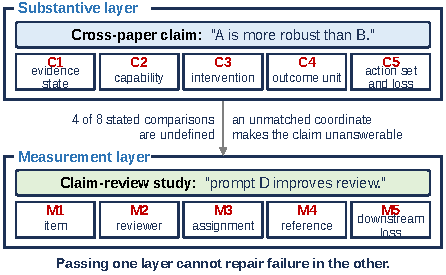
\includegraphics[width=\columnwidth]{figures/generated/fig_two_layer.pdf}%
\caption{The two layers answer different questions about the same sentence.
The substantive layer asks whether two published results concern one decision
problem; Table~\ref{tab:cross-paper-cases} applies it to real comparisons and
supplies the four-of-eight count. The measurement layer asks what a study of
claim review estimates; Table~\ref{tab:retrospective-remedies} shows which
analyses of such a study are valid. Passing one layer cannot repair failure in
the other.}
\label{fig:two-layer}
\end{figure}


\paragraph{Decision rule.}
For a proposed comparison, record each coordinate on both sides from the
sources alone. If every coordinate matches, the quoted gap stands. If a
coordinate differs but one side reports an operating point at the other side's
setting, re-read the comparison at that matched point and report the matched
number. If a coordinate differs and no matched operating point exists, the gap
is undefined and the comparison must be replaced by the common scope both
studies support, or dropped. \S\ref{sec:cases} applies exactly this rule.

\paragraph{Three targets.}
A majority-label difference for two realized reviewer panels is a
\emph{panel contrast}. A prompt effect over reviewers instead averages
individual potential judgments over a defined participant and item population.
A claim of better decisions requires a third target: expected downstream loss
for accepting, narrowing, rejecting, or deferring a comparison. These targets
coincide only under assumptions that should be stated rather than inherited
from the aggregation rule. Appendix
Section~\ref{sec:estimand-formalization} gives the notation.

\paragraph{Assignment and reference.}
Source resampling with reviewers fixed measures item variation conditional on
the realized panel; if prompts are assigned to reviewers, reviewer-composition
variation remains as claims accumulate, so more labels per person improve
conditional precision without creating new prompt assignments. Separately,
blinding reference writers to arm responses prevents copying, but a rubric that
paraphrases the tested prompt still embeds the intervention. We therefore say
``reference-relative agreement,'' reserving ``accuracy'' for an
intervention-independent criterion.

\section{Twelve Published Comparisons}
\label{sec:cases}

We assembled comparisons of two kinds from 259 locally extracted full texts:
\emph{direct} (eight cases), where one paper reports its own number beside a
number attributed to another paper, and \emph{survey-invited} (four), where a
survey or benchmark groups two systems under one label so that a reader would
rank their headline numbers. Every value is copied verbatim with a file and
line range, and \texttt{verify\_cross\_paper\_cases.py} re-opens each range and
fails on any mismatch; 70 checks pass. Ten of twelve do not survive as stated:
six have no common scope and four hold only on a strict subset. The most
frequently violated coordinate is the evidence state (10 of 12), followed by
the outcome unit (8) and origin/capability (5). We also audited three
within-harness contrasts, in which one paper compares systems under its own
corpus, retriever, generator and metric; two pass unchanged and one narrows
(Appendix Table~\ref{tab:cross-paper-cases-full}).

\paragraph{Capability envelopes decide security comparisons.}
All five security cases involve an unmatched attacker capability or objective.
Beyond the budget reversal in \S1, PoisonedRAG's 97\% is also quoted against a
corpus-poisoning attack whose reported quantity is a retrieval hit rate rather
than an answer-level success rate, so matching the budget alone moves the gap
from $0.96$ to $0.47$ without making the numbers commensurable. In the defense
direction, RobustRAG's certificate is stated at a corruption budget of one
passage, where the attack it is quoted as neutralizing succeeds $48\%$ rather
than $97\%$: ``reduces attack success from 97\%'' overstates the threat the
certificate covers. AIP's advantage over PoisonedRAG narrows rather than
dissolves, surviving at a matched budget on the shared domain only.

\paragraph{Outcome units decide noise comparisons.}
``Noise robustness'' names at least two measurements. RGB scores ChatGPT at
$76.00\%$ under a substring-match accuracy at a stated noise ratio; RAAT
scores ChatGPT-3.5 at $71.47$ exact match under a mixture of three
constructed noise types with the gold passage always present. The apparent
$4.53$-point gap combines a difference in metric strictness with a difference
in what counts as noise, and neither paper reports the other's metric, so the
gap does not even have a determined sign.

\paragraph{Matched comparisons survive.}
The audit does not flag everything. CRAG's self-corrective variant is compared
with Self-RAG at the same backbone, retriever, dataset and metric, and the
$6.9$-point gap stands. AstuteRAG evaluates RobustRAG's keyword-aggregation
variant inside its own harness with one model and one retrieval setup, and the
$4.4$-point gap stands as an accuracy comparison, with the caveat that
RobustRAG's certification guarantee is not what is being measured. Two of the
three within-harness controls likewise pass unchanged. A comparison lens that rejected
these would be useless.

\paragraph{Scope.}
These are cases, not a census. They were selected for the availability of both
sides in local full text and for the presence of an explicit number, which
favors open-access and widely cited work. They establish that the failure mode
occurs, that it is decisive, and that it is sometimes repairable from the
sources themselves; they do not estimate how often it occurs in the
literature.

\section{What Published Human Evaluations Report}
\label{sec:published-audit}

Deciding cases like these is a judgment task, so we asked what would be needed
to study it. Of 39 venue- or proceedings-linked Map B papers with locally
extracted full text, a deterministic human-judgment term screen flagged 19,
and full-text eligibility review retained nine that collected original human
judgments. The released ledger records the exact text lines supporting every
coding decision.

Two of nine papers report the number of distinct annotators. Two report both
raters per item and the number of items ($R=2$ and $P=2$ in Appendix
Table~\ref{tab:published-human-evaluation-audit}), four report an agreement or
rater-uncertainty quantity, and two report compensation. None reports the
item--annotator assignment, none releases pre-aggregation votes, and none
randomizes an audit prompt across annotators, so this audit finds no
verifiable assignment-unit mismatch. Absent fields are coded as reporting
gaps, not as evidence that a practice was absent. The screen is narrow and
single-coded and establishes concrete cases, not prevalence; the
under-reporting finding itself is already established at scale by
\citet{howcroft2020twenty} and \citet{vanderlee2021human}.

The specific increment is that the missing fields are exactly the ones a
reanalysis needs. FaithEval reports three crowd workers per pair with majority
inclusion \citep{rrag040}; RAGTruth reports two annotators per response, a
third reviewer for large differences, and \$25 per hour \citep{ragTruth2024};
ParamMute reports six senior researchers and a multiply annotated 100-item
subset but not their allocation to items \citep{rrag024}; PoisonedRAG names the
authors as evaluators without reviewer-level multiplicity
\citep{poisonedRAG2024}. In every case the released artifact is a final
aggregated label, enough to report an agreement rate and not enough to
recompute uncertainty at the unit that was assigned.
\S\ref{sec:simulation} prices that difference.

\subsection{Development diagnostic and its negative result}
\label{sec:development}

We also asked whether the coordinates can be used directly as a coding
instrument. In a development diagnostic, three coders reviewed 80 comparison
claims and a fourth adjudicated them with model labels hidden. Coder agreement
is uneven across coordinates: the policy/utility field is the most reliable
(pairwise $\kappa$ up to $.737$, Gwet's $AC_1$ up to $.913$) and the evidence
state the least ($\kappa$ $.101$--$.283$), with control status similarly low.
Only 39/80 verdicts were unanimous.

Appendix Table~\ref{tab:rule-baselines} reports what those figures are worth
against the baselines a classifier must beat. The full rule reaches $.500$
exact agreement, below the $.537$ obtained by predicting the modal adjudicated
verdict, and adding the C2 and C5 coordinates to the ablation shifts exact
agreement by $.000$ (95\% CI $[-.066, +.079]$, exact McNemar $p=1.0$); the
five-coordinate variant reaches $.550$, which is also inside the majority-class
interval. The sample overlaps codebook development and has a recoverable
selection rule for only 16 items. We therefore state the negative result
plainly: this diagnostic gives no evidence that the coordinates work as a
four-way classifier, and the substantive evidence in this paper is the
source-linked case analysis of \S\ref{sec:cases}, not an instrument claim.

A later 480-claim protocol is retained only as a design case. One returned
batch contained shared response payloads, and a later export could not be
linked to controlled recruitment records, one-to-one pseudonym mappings, and
separate response receipts available to the research team or an authorized
auditor. We therefore exclude every response, contrast, reference statistic,
participant attribute, and timing claim derived from it. Public identity
disclosure is neither required nor desirable; the missing element was an
internal audit trail, not public identifiers. The Ethics Statement gives the
disclosure in full.

\section{A Controlled Consequence Test}
\label{sec:controlled-models}

The two least conventional coordinates are origin/capability (C2) and
policy/utility (C5), and the case analysis shows both doing real work. We
therefore ask whether naming them changes a deployment decision, using a
target that no human supplies.

\paragraph{Benchmark.}
A deterministic benchmark contains 600 synthetic deployment decisions in 300
counterfactual pairs, in three strata. In \emph{C2} (120 pairs) only whether
the deployed origin, access, and budget fall inside an evaluated capability
envelope changes; half the pairs move both systems out of their envelopes and
half move only one, so a capability shift can flip the ordering between
systems rather than always resolving into deferral. In \emph{C5} (120 pairs)
only the error-versus-abstention prices or the exogenous price of commissioning
a further study changes; the deferral price is displayed as a constant rather
than derived from the deployment losses, so deferring is optimal on 65 of 240
items and the stratum is a genuine three-way decision. A \emph{competence
probe} (60 pairs) displays all three action losses directly and asks for the
minimum. The target is always the unique minimum of the displayed loss rule,
with a margin of at least $.02$; targets are balanced across the three actions
within every stratum, so no stratum is solvable by a constant response.

\paragraph{Design.}
Each model answers every item under three arms crossed with four hand-written
paraphrases, i.e.\ 7{,}200 greedy decisions per model. The \emph{ablated} arm
asks for evidence state, intervention, outcome, controls, and action. The
\emph{full} arm adds explicit origin/capability and policy/utility checks. The
\emph{placebo} arm adds generic reading instructions of matched length that
name neither coordinate, so that \emph{full} minus \emph{placebo}---our
primary contrast---is not confounded with instruction verbosity. Paraphrases
vary wording, ordering, voice and layout. Uncertainty is a bootstrap clustered
on the 300 counterfactual pairs, which is the unit the benchmark varies; the
grid of gate-passing models by stratum receives a Holm correction, and models
are combined by a random-effects meta-analysis so the reported effect refers
to a model population.

\paragraph{Validity gate.}
A model enters the primary analysis only if it reaches 50\% on the competence
probe in at least one arm and does not emit a single action on more than 90\%
of items. This rule was fixed before the runs. It exists because a constant
predictor is not performing the task, and counting one as evidence about
prompt sensitivity would be a category error.

\begin{table}[t]
\centering\footnotesize
\setlength{\tabcolsep}{1.5pt}
\resizebox{\columnwidth}{!}{%
\begin{tabular}{@{}lrrr@{}}
\toprule
Developer (models) & Probe & C2 $\Delta$ & C5 $\Delta$ \\
\midrule
01.AI (1) & +12.3 & -5.2 & +2.5 \\
AI2 (2) & +2.3 & -4.3 & -1.6 \\
Alibaba (5) & -0.2 & +10.4 & +2.1 \\
Anthropic (2) & +0.4 & -2.3 & -7.0 \\
Google (2) & +0.9 & +6.6 & -3.2 \\
HuggingFace (2) & -0.1 & +2.7 & -3.7 \\
IBM (2) & -3.9 & -1.3 & +0.1 \\
Meta (1) & -4.8 & +5.6 & -3.5 \\
Microsoft (2) & -0.4 & +10.2 & +3.1 \\
Mistral (2) & -7.0 & -0.6 & +0.0 \\
NVIDIA (1) & +1.0 & +4.7 & -2.0 \\
TII (2) & -1.8 & +1.7 & +5.0 \\
Zhipu (1) & -0.8 & -4.7 & +5.4 \\
\midrule
Pooled (random effects) & -0.4 & +3.1 & +0.1 \\
\quad 95\% CI & [-1.2, +0.4] & [+0.7, +5.5] & [-1.3, +1.5] \\
\quad 95\% pred. & [-4.4, +3.6] & [-9.8, +16.0] & [-7.2, +7.3] \\
\quad $I^2$ & 90\% & 98\% & 97\% \\
\quad dev.\ level & +0.1 & +1.7 & +0.4 \\
\bottomrule
\end{tabular}}
\caption{Controlled consequence test, \emph{full} minus \emph{placebo} in accuracy points, aggregated by developer. Checkpoints are nested in developers, so the developer-level row averages within developer before pooling. The prediction interval, not the confidence interval, is the quantity relevant to a claim about a model population; it contains zero on both substantive strata. The competence probe is the negative control. Per-model contrasts, Holm-adjusted values, paraphrase spread and the decision-normalisation report are in Appendix Table~\ref{tab:controlled-model-judges-strata-v2}.}
\label{tab:controlled-model-judges-v2}
\end{table}


\paragraph{Results.}
\CMJmodels{} instruction-tuned open models from five developers were run;
\CMJpassing{} passed the validity gate and \CMJfailing{} did not, with
competence-probe accuracy ranging from \CMJprobeMin\% to \CMJprobeMax\%.
Across gate-passing models the pooled \emph{full} minus \emph{placebo} effect
is \CMJCtwoPooled{} points on the capability stratum
(95\% CI [\CMJCtwoLow, \CMJCtwoHigh], $p\,\CMJCtwoP$, $I^2=\CMJCtwoIsq\%$) and
\CMJCfivePooled{} points on the utility stratum
(95\% CI [\CMJCfiveLow, \CMJCfiveHigh], $p\,{=}\,\CMJCfiveP$). Appendix
Table~\ref{tab:controlled-model-judges-strata-v2} gives the per-model
contrasts, paraphrase spread, and Holm-adjusted values.

The competence probe is the internal negative control. Its items are decided
by comparing three displayed losses, so naming a coordinate should not help,
and it does not: the pooled effect there is \CMJProbePooled{} points
(95\% CI [\CMJProbeLow, \CMJProbeHigh], $p\,{=}\,\CMJProbeP$). An arm effect
concentrated on the strata where the coordinate is decisive, and absent where
it is not, is what construct evidence for a coordinate should look like.

Two design points follow. The placebo arm matters: comparing \emph{full}
against \emph{ablated} conflates coordinate naming with roughly eighty extra
tokens of instruction, and the two contrasts do not agree. And between-model
heterogeneity is large ($I^2$ above 90\% on both substantive strata), which is
exactly why a single-checkpoint result would have been uninformative. These
are executable construct evidence about what naming a coordinate does to a
model's deployment choice; they are not evidence about human auditors and do
not validate the coordinates as a coding instrument.

\section{Pricing the Reporting Gap}
\label{sec:simulation}

\subsection{How heterogeneous are reviewers?}

The consequence of analyzing at the wrong unit depends on how much reviewers
differ. That quantity, $\sigma_r$, is the between-reviewer standard deviation
of ability on the logit scale, and it is identified only by a design that
crosses reviewers with items. We estimate it from the one such design
available to us, the retained 80-claim diagnostic, whose three coders each
labelled all 80 claims against an independent adjudication. A moment estimator
that removes the binomial sampling component gives $\hat\sigma_r = 0.27$, with
a source-clustered bootstrap 50\% interval of $[0.23, 0.40]$ and 95\% interval
of $[0.00, 0.53]$. Three raters make a variance imprecise, so the interval is
the estimate.

We then asked whether the published literature could do better. Two audited
papers report a rater-agreement rate: RAGTruth reports 91.8\% response-level
consistency between two annotators, and FaithEval reports over 98\% agreement
under majority voting. Under the same latent model, a reported pairwise
agreement constrains the total latent dispersion but not its split between
reviewer and item components. At the label prevalence those papers imply,
every $\sigma_r$ on a $0$--$1.2$ grid reproduces the reported agreement for
some item dispersion: the reported statistic places no usable restriction at
all (Appendix Table~\ref{tab:reviewer-heterogeneity-anchor}). Separating the
components requires the item--annotator assignment, which no audited paper
reports. The sweep below is therefore not a stylistic choice; it is what the
available reporting permits.

\subsection{Design}

We simulate a two-arm claim-review study with twelve reviewers, six per
prompt, $G$ sources contributing six claims each, and a balanced three-of-six
panel per claim in both arms. Baseline agreement is 75\%; source and claim
logit standard deviations are $.15$ and $.35$. Reviewer abilities are redrawn
from $N(0,\sigma_r^2)$ in every replicate, so the target is a
reviewer-population effect and the source-only analysis cannot be defended as
answering a realized-panel estimand instead; Appendix
Table~\ref{tab:retrospective-remedies-full} repeats everything with abilities
held at fixed population quantiles, with the same conclusions. Each cell uses
5,000 replicates at $\alpha=.05$, under a sharp null and under a true prompt
effect of $0.4$ logits.

Four analyses are compared. \emph{Panel/src} is the status quo: a paired source
$t$ test on panel-majority correctness, computable from released majority
labels alone. \emph{Votes/src} keeps the source-level standard error but uses
individual votes. \emph{Rev.\ $t$} is a two-sample $t$ test on the twelve
individual reviewer accuracies, and \emph{Rev.\ RI} refers that contrast to all
$\binom{12}{6}=924$ arm assignments. The last two need only pre-aggregation
votes carrying reviewer identifiers, so unlike an oracle test over a complete
vote matrix they are executable after collection.

\begin{table}[t]
\centering\footnotesize
\setlength{\tabcolsep}{2.6pt}
\begin{tabular}{@{}lrrrr@{}}
\toprule
Setting & Panel/src & Votes/src & Rev.\ $t$ & Rev.\ RI \\
\midrule
\multicolumn{5}{@{}l}{\emph{Size: no prompt effect, $\alpha=.05$}} \\
$\sigma_r=0.00$, $G=80$ & 4.7 & 5.1 & 4.7 & 4.3 \\
$\sigma_r=0.27$, $G=80$$\;\ast$ & 24.2 & 32.9 & 4.6 & 4.3 \\
$\sigma_r=0.78$, $G=80$ & 62.6 & 70.1 & 5.1 & 5.0 \\
$\sigma_r=0.27$, $G=160$ & 36.7 & 46.5 & 4.4 & 4.3 \\
\midrule
\multicolumn{5}{@{}l}{\emph{Power: true prompt effect $0.4$ logits}} \\
$\sigma_r=0.27$, $G=80$ & 78.8 & 89.0 & 52.8 & 51.6 \\
$\sigma_r=0.78$, $G=80$ & 69.6 & 77.0 & 11.4 & 11.4 \\
\bottomrule
\end{tabular}
\caption{Rejection percentages over 5,000 replicates with twelve reviewers, six per prompt, six claims per source $G$, and balanced three-of-six panels. Reviewer abilities are redrawn every replicate, so the target is a reviewer-population effect rather than a realized-panel contrast. $\sigma_r$ is the between-reviewer ability standard deviation on the logit scale; the starred row is the value estimated from the crossed three-coder diagnostic ($\hat\sigma_r=0.27$, Appendix Table~\ref{tab:reviewer-heterogeneity-anchor}). \emph{Panel/src} is the status-quo paired source $t$ test on panel-majority correctness; \emph{Votes/src} keeps the source-level standard error but uses individual votes; \emph{Rev.\ $t$} is a two-sample $t$ test on the twelve individual reviewer accuracies; \emph{Rev.\ RI} refers the same contrast to all 924 arm assignments. The last two are executable retrospectively from released pre-aggregation votes with reviewer identifiers, and retain power. The complete grid over both reviewer-ability profiles (fixed quantiles and resampled), all heterogeneities and all source counts is released as \texttt{supplement/retrospective\_remedy\_simulation.json}.}
\label{tab:retrospective-remedies}
\end{table}

\begin{figure}[t]
\centering
\resizebox{\columnwidth}{!}{%
\begin{tikzpicture}[font=\scriptsize]
\draw[->] (0,0) -- (0.89\columnwidth,0) node[right, xshift=-2pt, yshift=-6pt] {$G$};
\draw[->] (0,0) -- (0,3.75cm);
\node[rotate=90, anchor=south] at (-0.06\columnwidth,1.70cm) {rejection rate (\%)};
\draw[black!15] (0,0.000cm) -- (0.86\columnwidth,0.000cm);
\node[anchor=east] at (-0.005\columnwidth,0.000cm) {0};
\draw[black!15] (0,0.971cm) -- (0.86\columnwidth,0.971cm);
\node[anchor=east] at (-0.005\columnwidth,0.971cm) {20};
\draw[black!15] (0,1.943cm) -- (0.86\columnwidth,1.943cm);
\node[anchor=east] at (-0.005\columnwidth,1.943cm) {40};
\draw[black!15] (0,2.914cm) -- (0.86\columnwidth,2.914cm);
\node[anchor=east] at (-0.005\columnwidth,2.914cm) {60};
\draw[black!45, densely dotted, thick] (0,0.243cm) -- (0.86\columnwidth,0.243cm);
\node[anchor=north] at (0.000\columnwidth,0) {20};
\node[anchor=north] at (0.287\columnwidth,0) {40};
\node[anchor=north] at (0.573\columnwidth,0) {80};
\node[anchor=north] at (0.860\columnwidth,0) {160};
\draw[black, solid, thick] (0.000\columnwidth,0.481cm) -- (0.287\columnwidth,0.716cm) -- (0.573\columnwidth,1.176cm) -- (0.860\columnwidth,1.783cm);
\node[black] at (0.000\columnwidth,0.481cm) {$\bullet$};
\node[black] at (0.287\columnwidth,0.716cm) {$\bullet$};
\node[black] at (0.573\columnwidth,1.176cm) {$\bullet$};
\node[black] at (0.860\columnwidth,1.783cm) {$\bullet$};
\draw[black!55, dashed, thick] (0.000\columnwidth,0.644cm) -- (0.287\columnwidth,1.044cm) -- (0.573\columnwidth,1.599cm) -- (0.860\columnwidth,2.260cm);
\node[black!55] at (0.000\columnwidth,0.644cm) {$\circ$};
\node[black!55] at (0.287\columnwidth,1.044cm) {$\circ$};
\node[black!55] at (0.573\columnwidth,1.599cm) {$\circ$};
\node[black!55] at (0.860\columnwidth,2.260cm) {$\circ$};
\draw[black, solid, thick] (0.000\columnwidth,0.232cm) -- (0.287\columnwidth,0.241cm) -- (0.573\columnwidth,0.222cm) -- (0.860\columnwidth,0.215cm);
\node[black] at (0.000\columnwidth,0.232cm) {$\bullet$};
\node[black] at (0.287\columnwidth,0.241cm) {$\bullet$};
\node[black] at (0.573\columnwidth,0.222cm) {$\bullet$};
\node[black] at (0.860\columnwidth,0.215cm) {$\bullet$};
\draw[black!55, dashed, thick] (0.000\columnwidth,0.181cm) -- (0.287\columnwidth,0.209cm) -- (0.573\columnwidth,0.210cm) -- (0.860\columnwidth,0.208cm);
\node[black!55] at (0.000\columnwidth,0.181cm) {$\circ$};
\node[black!55] at (0.287\columnwidth,0.209cm) {$\circ$};
\node[black!55] at (0.573\columnwidth,0.210cm) {$\circ$};
\node[black!55] at (0.860\columnwidth,0.208cm) {$\circ$};
\node[anchor=east, font=\tiny] at (0.86\columnwidth,2.06cm) {panel majority, source SE};
\node[anchor=east, font=\tiny, black!55] at (0.86\columnwidth,2.54cm) {individual votes, source SE};
\node[anchor=west, font=\tiny] at (0.02\columnwidth,0.50cm) {reviewer-level $t$ / randomization};
\end{tikzpicture}}
\caption{Null rejection rate against the number of sources $G$ at the estimated reviewer heterogeneity $\sigma_r=0.27$, with reviewer abilities redrawn each replicate. Adding sources makes the two source-level analyses steadily worse, and using individual votes instead of majority labels does not help: the defect is the unit of uncertainty, not the aggregation. The two reviewer-level analyses stay at the nominal level and are executable from released pre-aggregation votes. Table~\ref{tab:retrospective-remedies} gives the values and the corresponding power.}
\label{fig:remedy-calibration}
\end{figure}


\subsection{Results}

At the estimated $\hat\sigma_r=0.27$ and 80 sources, the status-quo analysis
rejects a true null 24.2\% of the time, and 36.7\% at 160 sources: adding
sources makes it worse, because conditional item precision improves while the
number of prompt assignments stays at twelve. Replacing majority labels with
individual votes does not help and in fact hurts, reaching 32.9\% at 80
sources. That comparison isolates the cause. The defect is the unit over which
uncertainty is computed, not the majority aggregation, which is why advice to
release pre-adjudication labels is necessary but not sufficient.

Both reviewer-level analyses hold the nominal level across the whole grid:
4.6\% and 4.3\% at $\hat\sigma_r=0.27$ and 80 sources, and 4.4\% and 4.3\% at
160 sources, with the same behavior at $\sigma_r$ up to $0.53$
(Figure~\ref{fig:remedy-calibration}). They are not merely conservative:
against a true prompt effect of $0.4$ logits they reject 52.8\% and 51.6\% at
80 sources, rising to 56.3\% and 55.4\% at 160. The valid analyses lose power
relative to the invalid ones, but that difference is the part of the apparent
precision that was never earned.

\paragraph{What an author of a collected study should do.}
Compute the effect at the reviewer level and report it two ways: a two-sample
test on individual reviewer accuracies, and its exact assignment permutation.
Both require only that pre-aggregation votes be released with stable reviewer
identifiers. Where reviewers are crossed with items, a mixed-effects model
with crossed reviewer and item intercepts targets the same estimand
\citep{baayen2008crossed,barr2013maximal}; our contribution is not that
recommendation but the demonstration that the simpler reviewer-level tests
already recover calibration in this design, and that the single artifact
blocking either of them is the one no audited paper releases.

\section{A Pre-Collection Checklist}
\label{sec:practical-audit}

The audit is cheapest before labels exist. Five decisions follow from
\S\ref{sec:cases}--\S\ref{sec:simulation}; Appendix
Table~\ref{tab:robust-rag-reporting-checklist} expands the reporting fields.
\emph{(1) Name the claim and decision.} The unit under review is an atomic
public statement, not a paper, and verifying source support, deciding
comparability, and recommending an action are three different targets.
\emph{(2) Draw the unit map.} List the item, reviewer, treatment-assignment,
scoring, reference, and generalization units together; if prompts are assigned
to people, people remain the treatment units after majority voting, and
claim-in-paper nesting adds a layer rather than replacing reviewer dependence.
\emph{(3) Construct the target independently.} A reference rubric must not
paraphrase the tested intervention; where possible generate the target from a
predeclared consequence such as deployment loss under matched capability and
cost assumptions, and prefer admissible sets to forced adjudication when the
sources are ambiguous. \emph{(4) Power the randomized units.} Vary the number
and heterogeneity of reviewers, not only the number of claims: if an interval
keeps shrinking while reviewers are held fixed, it is conditional on the panel
\citep{card2020power}. Our $\hat\sigma_r=0.27$ is a usable starting value.
\emph{(5) Preserve the measurement path.} Release pre-adjudication votes with
stable reviewer identifiers, class supports, abstentions, unresolved cases, and
aggregation rules. \S\ref{sec:simulation} shows that this single artifact is
what makes a valid retrospective analysis possible; majority labels alone do
not. Hashes establish which bytes were analyzed, not that nominally distinct
people acted independently, and unverifiable provenance requires exclusion
rather than statistical repair.

\paragraph{A prospective human test.}
A corrected experiment would randomize enough independent participants between
prompts, or cross participants with prompts under counterbalancing and
carryover controls, analyze at the assignment unit, and model participant,
item, and reference-rater variation, with the protocol externally timestamped
before outcomes \citep{vanmiltenburg2021preregistering}. The benchmark of
\S\ref{sec:controlled-models} supplies an intervention-independent target;
\S\ref{sec:simulation} supplies the analysis plan and a starting value for the
power calculation.

\section{Conclusion}

Robust RAG is not a single leaderboard, and the cost of pretending otherwise is
measurable. Ten of twelve cross-paper comparisons drawn from published
robust-RAG work do not survive a five-coordinate audit as stated, and in the
sharpest case a quoted $3.7$-point attack-success lead reverses to $-45.3$
points once both sides are read at a matched insertion budget. Two of three
within-harness contrasts pass unchanged, so the coordinates discriminate
rather than condemn. Matching capability envelopes and outcome units is not a
methodological nicety; it decides orderings.

Deciding such claims with human reviewers is itself a measurement problem, and
the field currently cannot check its own answers. None of the nine robust-RAG
papers that collect original human judgments reports the item--annotator
assignment or releases pre-aggregation votes. That is not a bookkeeping
complaint: at the reviewer heterogeneity we estimate, the analysis those
papers make possible rejects a true null roughly a quarter of the time at 80
sources and gets worse as items accumulate, while two reviewer-level analyses
hold the nominal level and keep power. Both are executable after collection
and both need exactly the artifact that is missing. Releasing per-reviewer
votes is therefore the single highest-value change available, and it costs
nothing.

We are equally clear about what is not shown: the coordinates are disclosure
fields validated on published comparisons, not a coding instrument, since on an
80-claim development sample no variant of the schema separates from predicting
the modal verdict.

\paragraph{Artifact availability.}
The supplement releases the source-linked comparability cases and their
verifier, the published-study ledger, the v2 benchmark, model outputs and
clustered analysis, the reviewer-heterogeneity estimator, and both
simulations. Every evidence-bearing table is linked to a machine-readable
source. Excluded outcome exports are omitted from release packages; a
privacy-safe invalidation receipt preserves the shared-payload finding and the
original return-manifest hash.

\section*{Limitations}

The twelve comparability cases are cases, not a census. Both sides had to be
present in local full text with an explicit number, which favors open-access
and widely cited work, and the coordinate-matched re-reading is available only
where a paper reports an operating point at the other side's setting; seven of
the fifteen entries record that no such value is recoverable from the text.
Coding of the cases is ours and single-coded, though every quoted value is
machine-verified against its source line. The cases show that the failure mode
occurs and can be decisive; they do not estimate its frequency.

The nine-paper reporting audit is a single-coded, model-assisted pass over 39
venue-linked local full texts. It is neither a scoping review conducted to
protocol \citep{prismaScR2018} nor a risk-of-bias assessment
\citep{whiting2011quadas}, and
the under-reporting phenomenon is established at larger scale elsewhere
\citep{howcroft2020twenty,vanderlee2021human}. Absence of a reported field is
not evidence of an absent practice, and later supplements or author records
could resolve fields marked unreported. The broader map is open-PDF based and
overrepresents English-language, openly accessible work.

The reviewer-heterogeneity estimate rests on three coders and 80 claims: the
bootstrap interval $[0.00, 0.53]$ is wide, and the point value $0.27$ should
be read as a starting value, not a field constant. The simulation uses binary
correctness, a common wrong-label state, balanced three-of-six panels, and a
logit random-effects model; it demonstrates a design failure mode and the
analyses that repair it, not a prevalence. The two reviewer-level remedies
require released per-reviewer votes; where reviewers rate disjoint item sets
they will be less efficient than a crossed mixed-effects model.

The controlled benchmark is templated arithmetic prose with a synthetic loss
rule. Open instruction-tuned checkpoints are a convenience sample of a model
population, results do not predict behavior on natural paper claims, and the
paraphrase set is four hand-written variants rather than a sampled template
population. The v1 benchmark was corrected after outcomes were observed
(a C2 generator also moved the deferral cost); v2 was rebuilt and every
reported model was rerun on it, so the v2 contrast is a fresh measurement but
the benchmark family is not preregistered.

The 80-claim diagnostic is purposive, overlaps codebook development, and lacks
a recoverable selection procedure for 64 items; its result is negative and is
reported as such. The excluded 480-claim collection lacks the internal
provenance needed for a human-study claim, and no quantity derived from it
appears anywhere in this paper, including the heterogeneity estimate. Local
hashes authenticate bytes, not behavioral independence or external
preregistration. No consequence-based human effect size is estimated.

\section*{Ethics Statement}

For the retained 80-claim diagnostic, the project owner attests that all four
contributors consented to paper use and public release of de-identified
annotations, including rationales, were compensated, and did not use
generative AI for annotation. The public provenance is that attestation rather
than contributor-level consent or identity records. The project owner also
reports an institutional determination that formal review was not required.

We make no human-subject, recruitment, expertise, compensation, or
independence claim for the excluded 480-claim collection. One returned batch
contained shared response payloads, and a later export could not be linked to
controlled recruitment records, one-to-one pseudonym mappings, and separate
response receipts. Because that internal audit trail was absent, every
response, contrast, reference statistic, participant attribute, and timing
claim derived from it is excluded, including from the reviewer-heterogeneity
estimate in \S\ref{sec:simulation}; a privacy-safe invalidation receipt
preserves the shared-payload finding and the original return-manifest hash. We
distinguish public de-identification from private auditability: consent,
recruitment, and identity-linkage records may remain access-controlled, but an
empirical claim still needs an inspectable internal provenance path. The
published-paper audit uses public scholarly documents and introduces no
participant contact. The comparability cases quote short passages from
published papers for verification purposes only. LLMs assisted documentary
discovery, extraction, and audit screening; those outputs are not human gold.
The synthetic benchmark contains no participant data or third-party
quotation. The reported open-model runs use deterministic decoding and release
raw outputs. No attack payloads or poisoned corpora are released.

\clearpage
\bibliography{references,auto_references,venue_authoritative_references,venue_extra_references,venue_200_selected_references,multimodal_100_selected_references}

\clearpage
\appendix

\section{Substantive Comparability in Robust RAG}
\label{sec:robust-rag-landscape}

We use the literature map as a source of boundary cases, not as prevalence
evidence. Five \emph{operating questions} organise discovery: how evidence is
constructed, how a model uses it, how deliberate corruption changes the game,
how signals become actions, and how those actions are evaluated. They are a
different cut of the same literature from the four failure surfaces of
\S\ref{sec:taxonomy}, and both are different again from the five
\emph{reporting coordinates} of \S\ref{sec:coordinates}, which describe not a
literature but a single proposed contrast. The boundary cases below are what
made the coordinates necessary.

\paragraph{Evidence availability is not evidence use.}
Irrelevant-context studies test whether retrieved distractors redirect a
generator \citep{irrelevantContext2023}; noise-aware training changes the
generator's training distribution \citep{raat2024}; RGB supplies diagnostic
stress conditions \citep{rgb2023}; and Chain-of-Note changes how retrieved
documents are read \citep{chainOfNote2023}. A filter, a trained reader, and a
benchmark may share a harness, but their native scores do not rank
interchangeable interventions. Insufficient evidence creates another
boundary: when no passage can support an answer, re-retrieval or abstention
can dominate better distractor resistance \citep{sufficientContext2024}.

\paragraph{Support, authority, conflict, and attack are distinct.}
RAGTruth annotates unsupported spans, while evaluators estimate claim or
response support \citep{ragTruth2024,ragas2024,ares2024}; knowledge-conflict
methods instead study competition between parametric memory and retrieved
evidence \citep{tugOfWar2024,faithfulRAG2025,astuteRAG2025}. A response can be
correct but unsupported, or faithful to a weak source. Provenance and timestamp
determine which source should govern \citep{kilt2021,freshllms2024,
realtimeQA2023}. Deliberate corruption changes the game again: corpus
poisoning, indirect prompt injection, and backdoors differ in corpus write
access, query knowledge, retriever visibility, insertion budget, persistence,
and objective \citep{poisonedRAG2024,aip2025,phantom2024}, and their defenses
prevent, detect, certify, trace, quarantine, or recover under different
assumptions \citep{certifiedRAG2024,rrag017,rrag128}. An attack-success
comparison is transportable only within a matched capability envelope.

\paragraph{A signal is not a policy.}
Calibration predicts a property of a score \citep{guo2017calibration};
selective prediction trades coverage against risk
\citep{geifman2017selective}; sufficient-context classification
asks whether available passages can support an answer; adaptive retrieval
chooses whether to search, verify, answer, or abstain
\citep{calibRAG2025,sufficientContext2024,whenToRetrieve2024}. Self-RAG, CRAG,
and CtrlA expose this policy layer explicitly
\citep{selfRAG2023,crag2024,ctrla2025}. Comparing them requires a common
action set, budget, and loss: accuracy alone cannot price extra retrieval,
coverage, or refusal.

\paragraph{Comparison ladder.}
The strongest contrast reruns alternatives with the same corpus snapshot,
retriever, generator, evidence state, capability envelope, action set, and
outcome. When that is impossible, synthesis should retain only the common
scope supported by both studies. If a decision-critical field is absent, the
comparison is under-specified rather than evidence that either method is
better. Appendix~\ref{sec:extended-survey} gives paper-level contrasts and the
documentary-map boundary; the next section turns these recurring boundaries
into a claim-level audit.


\section{Extended Synthesis by Operating Question}
\label{sec:extended-survey}

Sections~\ref{sec:evidence}--\ref{sec:system} organise robust RAG by failure
surface, which is where a paper sits. This appendix cuts the same literature the
other way, by the \emph{operating question} a study answers, and develops the
paper-level contrasts the main text compresses. It is a synthesis, not an
exhaustive bibliography: the released \MapRows{}-row evidence map holds the long-tail
records, source strata and intervention labels.

Two limits carry over from \S\ref{sec:protocol} and govern how the contrasts
below may be read. The screening flow's first stage is documented but not
re-executable, so this synthesis identifies recurring scientific distinctions
rather than estimating prevalence or ranking evidence families; and the map
carries no study-level risk-of-bias weighting. A review-directed recall check
also surfaced older, pre-freeze publications absent from the frozen map, which
we cite as qualitative context and log as post-freeze discoveries without
entering them into any denominator. Where this survey states a number rather
than a distinction, it does so only for the frame of \S\ref{sec:applied}.

\subsection{When Does Retrieved Context Help?}

Irrelevant-context and noise-aware-training studies intervene at different
points. \citet{irrelevantContext2023} shows that retrieved distractors can
actively redirect generation and tests filtering and targeted fine-tuning.
\citet{raat2024} instead trains a generator across random, relevant, and
counterfactual retrieval conditions. RGB supplies stress conditions and
diagnostic abilities rather than a competing mitigation \citep{rgb2023}.
These papers can share an end-to-end harness, but their native results do not
rank a filter, a trained reader, and a benchmark as interchangeable objects.

Context construction creates a second boundary. Chain-of-Note changes how the
generator reads retrieved documents, whereas compression and reranking alter
what reaches it \citep{chainOfNote2023,rrag044,rrag058}. Long-context studies
show that retaining more passages can improve evidence availability while
worsening position sensitivity or distraction \citep{rrag039,rrag143}. A fair
comparison therefore fixes the candidate evidence, generator, decoding, and
budget when the intended claim is about the intervention rather than the
entire system.

Insufficient evidence is not merely severe distraction. Sufficient Context
labels whether the available passages can support an answer and evaluates
selective behavior \citep{sufficientContext2024}. A reader that resists a hard
negative and a controller that abstains when support is absent solve different
problems. Reports should state both answer-bearing support availability and
the scored action.

\subsection{Which Knowledge Should Govern an Answer?}

Knowledge-conflict work separates context--memory disagreement from conflict
among retrieved sources. Tug-of-War measures how models trade parametric and
contextual knowledge; FaithfulRAG models fact-level discrepancies; Astute RAG
reconciles imperfect retrieval with internal knowledge
\citep{tugOfWar2024,faithfulRAG2025,astuteRAG2025}. Although all three concern
``conflict,'' their experimental units, source assumptions, and desired
responses differ. The appropriate outcome may be answer correctness,
contextual faithfulness, calibrated disclosure, or source reconciliation.
Earlier entity-substitution experiments and PopQA isolate when parametric
memory resists or benefits from retrieved evidence
\citep{longpre2021conflicts,mallen2023trust}. ConflictBank broadens the
benchmark unit to millions of claim--evidence pairs across misinformation,
temporal conflict, and semantic ambiguity \citep{conflictBank2024}; its scale
does not make those conflict types interchangeable.

Grounding resources address another layer. RAGTruth provides span-level
hallucination labels, while RAGAS and ARES estimate response or context support
\citep{ragTruth2024,ragas2024,ares2024}. These evaluators can identify an
unsupported answer, but support alone does not establish that the cited source
is current or authoritative. A system can be faithful to weak evidence or
correct for a reason absent from its citations.

Source reliability and time therefore belong in the evidence record. Recent
work models source reliability directly \citep{sourceReliabilityRAG2025}, and
other studies examine source preference and contextual authority
\citep{rrag132,rrag147}. The comparison-relevant question is not only whether
the model used retrieved text, but whether the benchmark specified which
source should govern, at what timestamp, and under what corroboration rule.
KILT standardizes provenance against a fixed knowledge source, while FreshQA
and RealTimeQA test knowledge whose answer changes over time
\citep{kilt2021,freshllms2024,realtimeQA2023}. ALCE and generative-search
verifiability work separately score citation attribution and whether cited
sources actually support generated statements
\citep{alce2023,verifiability2023}.

Multi-agent methods add yet another intervention boundary. MAIN-RAG uses
agent voting to filter retrieved documents, MADAM-RAG assigns agents to
conflicting documents before aggregation, and DRAG introduces debate during
retrieval and generation \citep{mainRAG2025,madamRAG2025,drag2025}. General
multi-agent debate supplies methodological background
\citep{duMultiagentDebate2024}, but these RAG systems should be compared only
when the evidence allocation, agent budget, aggregation rule, and target
outcome match.

\subsection{What Changes Under an Attacker?}

Corpus poisoning makes evidence unreliability intentional. PoisonedRAG inserts
passages to steer target answers; earlier corpus-poisoning work manipulates
retrieval through adversarial passages
\citep{poisonedRAG2024,poisoningRetrievalCorpora2023}. Attack success is
conditional on corpus write access, insertion budget, query knowledge,
retriever visibility, and target scope. Omitting these fields can make two
attack rates numerically similar but scientifically incomparable.

Indirect prompt injection and backdoors target a different interface.
Retrieved text may contain instructions that override the user task, or a
trigger may activate behavior learned during training
\citep{aip2025,phantom2024,trojanRAG2024}. These attacks should not inherit
claims from factual poisoning merely because both place malicious text in the
context. Retrieval realism, instruction-following behavior, and trigger access
define distinct games.

Defenses likewise have different roles. Certified RAG gives guarantees under a
bounded corruption model; filtering and semantic isolation demote suspicious
documents; traceback identifies likely poisoned sources
\citep{certifiedRAG2024,rrag017,rrag128}. Prevention, certified accuracy,
detection, and recovery require different outcomes. Any cross-defense
comparison should pair the same capability envelope with clean utility and
state whether the defense prevents, detects, traces, quarantines, or recovers.

\subsection{How Does a Signal Become an Action?}

Calibration, answerability, and retrieval usefulness are related but not
identical signals. Calibration-oriented RAG predicts reliability, whereas
Sufficient Context asks whether the retrieved evidence can support an answer
\citep{calibRAG2025,sufficientContext2024}. A well-calibrated score can still
feed a poor threshold or action policy, and an insufficient-context detector
does not determine whether retrieval, clarification, or abstention has the
highest utility.

Adaptive systems make the policy explicit. Self-RAG learns when to retrieve
and critique; CRAG adds corrective retrieval; CtrlA separates uncertainty
sources to select control actions
\citep{selfRAG2023,crag2024,ctrla2025}. Their reported gains depend on the
available action set and resource budget. Answer-only accuracy cannot capture
the benefit or cost of extra retrieval, verification, or refusal.

Selective evaluation should therefore retain risk, coverage, action, and cost
rather than collapse them into one score. Trust-or-abstain methods, conformal
controllers, and uncertainty benchmarks instantiate different operating
points \citep{rrag002,rrag041,rrag001}. Comparisons are strongest when systems
share evidence and actions and are evaluated across a risk--coverage or
utility curve.

\subsection{What Can the Evidence Map Establish?}

The map documents that robust-RAG research spans evidence construction,
evidence use, adversarial integrity, and action control. Existing surveys
provide architectural, evaluation, trustworthiness, security, conflict, and
abstention views
\citep{ragSurvey2024,ragEvaluationSurvey2024,trustRAGCompass2024,
securityRAGSurvey2026,xuKnowledgeConflicts2024,wenAbstentionSurvey2025}.
Controlled searches for RAG best practices provide an empirical component
comparison under shared tasks \citep{ragBestPractices2024}, complementary to
survey taxonomies and to the claim-level audit studied here.
Table~\ref{tab:main-prior-work-comparison} states the narrower claim-level
increment tested here.

The map cannot establish that these families occur at representative rates,
that its taxonomy is complete, or that one family has stronger evidence.
Accepted-paper additions strengthen several historical lines, while
\MapPreprints{} of \MapRows{} mapped rows remain preprints against
\MapPeerReviewed{} peer-reviewed, and coding depth varies across legacy strata.
Map counts therefore provide documentary context only. Every measured claim in
this survey rests elsewhere: the taxonomy test on the constructed benchmark of
\S\ref{sec:tested}, the composition figures on the screened frame of
\S\ref{sec:applied}, and the design claim on the assignment-unit simulation.


\section{Development Diagnostic Details}
\begin{table}[t]
\centering\scriptsize
\setlength{\tabcolsep}{2.5pt}
\begin{tabular}{@{}lrrl@{}}
\toprule
Estimator & Exact & $\kappa$ / $p$ & 95\% CI \\
\midrule
Three-field taxonomy & 0.300 & -0.003 & [0.182, 0.415] \\
Ablation (no C2/C5) & 0.500 & 0.254 & [0.390, 0.594] \\
Five coordinates & 0.550 & 0.315 & [0.494, 0.609] \\
Five coord.\textbackslash\{\} + controls & 0.500 & 0.273 & [0.420, 0.571] \\
Majority class (valid)$^{\dagger}$ & 0.537 & 0.000 & [0.432, 0.646] \\
Random (marginal)$^{\dagger}$ & 0.427 & 0.000 & [0.355, 0.519] \\
Uniform over 4 verdicts$^{\dagger}$ & 0.250 & 0.000 & -- \\
\midrule
\multicolumn{4}{@{}l}{\emph{Paired contrasts (source-clustered bootstrap)}} \\
Full $-$ Ablation & +0.000 & 1.00 & [-0.066, +0.079] \\
5-coord $-$ Ablation & +0.050 & 0.42 & [-0.029, +0.158] \\
Full $-$ Majority & -0.037 & 0.76 & [-0.163, +0.097] \\
5-coord $-$ Majority & +0.013 & 1.00 & [-0.099, +0.138] \\
\bottomrule
\end{tabular}
\caption{Development diagnostic on 80 comparison claims, with the trivial baselines ($\dagger$) the schema must beat. Intervals are percentile bootstrap intervals clustered on the source paper. No rule variant separates from the strongest trivial baseline (Majority class (valid), 0.537), and adding the C2 and C5 coordinates to the ablation moves exact agreement by an amount whose interval spans zero. The diagnostic therefore supplies no evidence that the coordinates work as a classifier, which is why the paper's substantive evidence rests on the source-linked comparability cases instead.}
\label{tab:rule-baselines}
\end{table}

\begin{table}[t]
\centering
\small
\setlength{\tabcolsep}{4pt}
\begin{tabularx}{\columnwidth}{Xr}
\toprule
\textbf{Human-validation diagnostic} & \textbf{Value} \\
\midrule
Model-stratum coverage (V/P/I/U) & 26/125; 25/134; 25/26; 4/4 \\
Unanimous verdicts & 39/80 \\
Adjudicator changes to available majorities & 9/78 \\
Pairwise verdict $\kappa$ & 0.258--0.525 \\
C1 / C3 / control-status $\kappa$ &
0.101--0.283 /
0.215--0.535 /
0.208--0.266 \\
Full-rule exact / $\kappa$ / macro-F1 &
0.500 / 0.273 /
0.437 \\
Model \emph{invalid} precision &
5/25 =
0.200 \\
\bottomrule
\end{tabularx}
\caption{Reliability diagnostics for the 80-claim human sample. V/P/I/U
denote the model-valid, partial, invalid, and under-specified strata; unequal
coverage and development overlap make these descriptive sample results, not
held-out population performance.}
\label{tab:main-human-validation}
\end{table}

\begin{table*}[t]
\centering
\small
\setlength{\tabcolsep}{5pt}
\begin{tabularx}{\linewidth}{Xccc}
\toprule
\textbf{Rule} & \textbf{Exact [95\% CI]} &
\textbf{$\kappa$ [95\% CI]} & \textbf{Macro-F1 [95\% CI]} \\
\midrule
Three-field taxonomy & 0.300 [0.182, 0.413] & -0.003 [-0.106, 0.109] & 0.180 [0.108, 0.256] \\
Evidence+controls (C2/C5 ablated) & 0.500 [0.389, 0.593] & 0.254 [0.079, 0.383] & 0.417 [0.247, 0.556] \\
Five coordinates & 0.550 [0.494, 0.612] & 0.315 [0.217, 0.393] & 0.382 [0.299, 0.449] \\
Five coordinates + controls & 0.500 [0.422, 0.575] & 0.273 [0.139, 0.364] & 0.437 [0.291, 0.547] \\
\bottomrule
\end{tabularx}
\caption{Agreement with adjudicated human verdicts on the 80-claim sample.
Intervals use 50,000 source-cluster bootstrap resamples
over nine sources. The resampling respects within-source dependence but cannot
make a non-probability, development-overlapping sample representative. All
rows still reuse the same model-coded fields.}
\label{tab:main-rule-reliability}
\end{table*}

\begin{table*}[t]
\centering
\small
\setlength{\tabcolsep}{6pt}
\begin{tabular}{lrrrr}
\toprule
\textbf{Human-adjudicated archetype} & \textbf{$n$} &
\textbf{Sources} & \textbf{Full exact [95\% CI]} &
\textbf{Full--ablated exact [95\% CI]} \\
\midrule
Self-baseline & 12 & 7 & 0.333 [0.111, 0.625] & +0.000 [+0.000, +0.000] \\
Shared harness & 22 & 5 & 0.500 [0.286, 0.737] & -0.045 [-0.150, +0.000] \\
Cross-source & 19 & 6 & 0.474 [0.217, 0.714] & +0.000 [-0.176, +0.214] \\
Causal/mechanistic & 14 & 5 & 0.500 [0.154, 0.846] & +0.000 [+0.000, +0.000] \\
Field-level & 5 & 2 & 0.600 [0.000, 0.750] & +0.000 [+0.000, +0.000] \\
Policy/utility & 8 & 5 & 0.750 [0.556, 1.000] & +0.125 [-0.333, +0.667] \\
\bottomrule
\end{tabular}
\caption{Exploratory archetype breakdown with source-cluster intervals.
Small strata and few source clusters yield wide or discrete intervals; the
rows should not be ranked as stable performance estimates.}
\label{tab:rule-reliability-by-archetype}
\end{table*}

\begin{table*}[t]
\centering
\small
\setlength{\tabcolsep}{6pt}
\begin{tabular}{lrrr}
\toprule
\textbf{Field} & \textbf{Raw agreement} &
\textbf{Cohen's $\kappa$} & \textbf{Gwet's AC1} \\
\midrule
Claim archetype & 0.637--0.738 & 0.546--0.659 & 0.570--0.690 \\
C1 evidence state & 0.375--0.550 & 0.101--0.283 & 0.256--0.470 \\
C2 origin/capability & 0.600--0.738 & 0.153--0.401 & 0.549--0.673 \\
C3 intervention & 0.537--0.787 & 0.215--0.535 & 0.438--0.727 \\
C4 outcome/unit & 0.662--0.750 & 0.253--0.462 & 0.620--0.718 \\
C5 policy/utility & 0.775--0.925 & 0.445--0.737 & 0.720--0.913 \\
Control status & 0.400--0.537 & 0.208--0.266 & 0.273--0.452 \\
Final verdict & 0.537--0.787 & 0.258--0.525 & 0.434--0.751 \\
\bottomrule
\end{tabular}
\caption{Ranges over the three human-coder pairs on all 80 claims. Low C1,
C3, and control-status agreement localises the main operational ambiguity.}
\label{tab:human-field-agreement}
\end{table*}

\begin{table}[t]
\centering
\small
\setlength{\tabcolsep}{4pt}
\begin{tabularx}{\columnwidth}{Xrrr}
\toprule
\textbf{Field} & \textbf{Exact} & \textbf{$\kappa$} &
\textbf{AC1} \\
\midrule
Archetype & 0.738 & 0.670 & 0.688 \\
C1 evidence state & 0.575 & 0.001 & 0.532 \\
C2 origin/capability & 0.725 & 0.359 & 0.679 \\
C3 intervention & 0.675 & 0.302 & 0.589 \\
C4 outcome/unit & 0.762 & 0.332 & 0.739 \\
C5 policy/utility & 0.887 & 0.705 & 0.861 \\
Control status & 0.562 & 0.356 & 0.474 \\
\bottomrule
\end{tabularx}
\caption{Agreement between model-coded fields and adjudicated human fields on
the same 80 claims. This separates field extraction/coding disagreement from
the later rule-composition step, although several intermediate rule flags were
not human-adjudicated.}
\label{tab:model-human-field-alignment}
\end{table}

\begin{table*}[t]
\centering
\small
\setlength{\tabcolsep}{6pt}
\begin{tabular}{lrrrrrr}
\toprule
\textbf{Reference labels} & \textbf{$n$} & \textbf{Ablated exact} &
\textbf{Full exact} & \textbf{$\Delta$ exact} &
\textbf{$\Delta\kappa$} & \textbf{$\Delta$ macro-F1} \\
\midrule
Adjudicated & 80 & 0.500 & 0.500 & +0.000 & +0.019 & +0.020 \\
Coder A & 80 & 0.475 & 0.463 & -0.012 & +0.007 & +0.015 \\
Coder B & 80 & 0.550 & 0.575 & +0.025 & +0.046 & +0.033 \\
Coder C & 80 & 0.438 & 0.400 & -0.037 & -0.020 & -0.016 \\
Available majority & 78 & 0.500 & 0.487 & -0.013 & +0.006 & +0.017 \\
Unanimous subset & 39 & 0.641 & 0.615 & -0.026 & -0.030 & -0.016 \\
\bottomrule
\end{tabular}
\caption{Sensitivity of the full-versus-ablated comparison to the reference
labels. Individual-coder, majority, and unanimous rows are pre-adjudication
diagnostics, not alternative gold standards. The sign of the exact-agreement
difference changes across references.}
\label{tab:reference-label-sensitivity}
\end{table*}


\FloatBarrier
\section{Comparability Case Ledger}
\label{sec:appendix-cases}
\begin{table*}[t]
\centering\scriptsize
\setlength{\tabcolsep}{3pt}
\begin{tabular}{@{}p{0.055\textwidth}p{0.30\textwidth}p{0.30\textwidth}p{0.29\textwidth}@{}}
\toprule
ID & Side A (reported value) & Side B (reported value) & Coordinate-matched reading \\
\midrule
SEC-01 & PoisonedRAG black-box ASR 0.97 on NQ, GPT-4, 5 injected texts per target question, Contriever retriever, top-5 context & Corpus Poisoning Attack ASR 0.01 on NQ as re-run by PoisonedRAG (Table 4)… & not\_recoverable\_from\_text \\
\addlinespace[1pt]
SEC-02 & PoisonedRAG black-box ASR 0.97 on NQ, 5 injected texts per target question, GPT-4, Contriever & Phantom attack success 93.3\% for Refusal-to-Answer on netflix trigger, Llama3-8B, Contriever, 1 poisoned document & PoisonedRAG ASR at 1 malicious text in top-5 = 0.48 on NQ black-box (Table 17 L2853-2856); Phantom = 93.3\% at 1 document \\
\addlinespace[1pt]
SEC-03 & RobustRAG: empirical ASR <=15\% in all cells of Table II; vanilla-RAG ASR for the poisoning attack 37.0-86.0 and for prompt injection 66.0-100… & PoisonedRAG black-box ASR 0.97 on NQ, 5 malicious texts injected per target question into a 2,681,468-text database, GPT-4, Contriever & Within RobustRAG's own harness the poisoning reduction is 86.0 $\rightarrow$ <=15.0 at its worst cell and 37.0 $\rightarrow$ <=12.0 on NQ (Table II, certifiedRAG2024.txt L1480-1485 and L1502-1507)… \\
\addlinespace[1pt]
SEC-04 & BadRAG MCOP 98.2\% attack success with 10 adversarial passages; GPT-4 reject ratio 74.6\% on NQ (denial-of-service) & PoisonedRAG black-box ASR 0.97 on NQ, GPT-4, 5 injected texts per target question & not\_recoverable\_from\_text \\
\addlinespace[1pt]
SEC-05 & AIP ASR 95.23\% on MedSquad, 5 adversarial documents, GPT-3.5-Turbo for rephrasing & PoisonedRAG ASR 28.57\% on MedSquad (as reported in AIP Table 1) & Both at 5 injected docs on MedSquad: AIP 95.23\% vs PoisonedRAG 28.57\% \\
\addlinespace[1pt]
NOISE-01 & Self-CRAG accuracy 61.8\% on PopQA, SelfRAG-LLaMA2-7b backbone & Self-RAG 7B accuracy 54.9\% on PopQA & Self-CRAG 61.8 vs Self-RAG 54.9 on PopQA (same backbone, retriever, metric) \\
\addlinespace[1pt]
NOISE-02 & CtrlA7B accuracy 61.8\% on PopQA, Mistral-7B, BM25+BGE retriever & Self-RAG 7B accuracy 54.9\% on PopQA, LLaMA2-7B, Contriever-MS MARCO & not\_recoverable\_from\_text \\
\addlinespace[1pt]
NOISE-03 & ChatGPT accuracy 76.00\% at 0.8 noise ratio on English QA subset & ChatGPT3.5 average EM 71.47 under mixed noise on RAG-Bench & not\_recoverable\_from\_text \\
\addlinespace[1pt]
NOISE-04 & Chain-of-Note EM 41.83 vs Retrieve-Read EM 34.28 on NQ at 100\% noise ratio, LLaMA-2 7B, DPR & RAAT EM 87.15 vs RALMmultiple EM 85.47 average across noise types, LLaMA2-7B, DPR & not\_recoverable\_from\_text \\
\addlinespace[1pt]
NOISE-05 & ASTUTE RAG accuracy 52.2\% on NQ, Claude 3.5 Sonnet, real-world retrieval & RobustRAG keyword aggregation accuracy 47.8\% on NQ, Claude 3.5 Sonnet (AstuteRAG Table 1) & ASTUTE RAG 52.2 vs RobustRAG 47.8 on NQ (matched LLM, dataset, metric) \\
\addlinespace[1pt]
FAITH-01 & Finetuned Llama-2-13B response-level hallucination detection overall F1 78.7\% & Same models at span-level (Table 6) — different and lower numbers for word-level localization & not\_recoverable\_from\_text \\
\addlinespace[1pt]
FAITH-02 & FaithfulRAG (mistral-7b-instruct) accuracy 81.7\% on FaithEval; Self-RAG (Llama2-7B) 37.4\% on FaithEval & GPT-4o 47.5\% accuracy on counterfactual context task of FaithEval; GPT-4o 96.3\% on closed-book QA & not\_recoverable\_from\_text \\
\addlinespace[1pt]
CALIB-01 & Self-RAG 7B accuracy 66.4\% on TriviaQA-unfiltered, Contriever-MS MARCO & Llama2-7B with retrieval accuracy 42.5\% on TriviaQA-unfiltered & Self-RAG 66.4 vs Llama2-7B RAG 42.5 on TriviaQA (all coordinates matched) \\
\addlinespace[1pt]
CALIB-02 & CtrlA7B accuracy 76.4\% on TriviaQA, Mistral-7B, BM25+BGE & FLARE accuracy 72.4\% on TriviaQA, reimplemented with Mistral-7B & CtrlA 76.4 vs FLARE 72.4 on TriviaQA (matched backbone, retriever, dataset) \\
\addlinespace[1pt]
CALIB-03 & ADAPT-LLM (SQuAD) accuracy 38.15\% on PopQA test set, Llama-2 7B, Contriever, exact match & Self-RAG 7B accuracy 54.9\% on PopQA long-tail subset (1,399 queries), Llama2-7B, Contriever-MS MARCO + web search & not\_recoverable\_from\_text \\
\addlinespace[1pt]
\bottomrule
\end{tabular}
\caption{Reported values and coordinate-matched readings for every comparability case. The released ledger records the file and line range supporting each value; the verifier re-opens each range and fails on any mismatch.}
\label{tab:cross-paper-cases-full}
\end{table*}


\FloatBarrier
\section{Published Human-Evaluation Audit Cases}
\begin{table}[t]
\centering\footnotesize
\setlength{\tabcolsep}{4pt}
\begin{tabular}{lrrrr}
\toprule
Reporting field & R & P & NR & N/A \\
\midrule
Distinct annotator count & 2 & 0 & 7 & 0 \\
Raters per item & 2 & 2 & 5 & 0 \\
Item--annotator assignment & 0 & 0 & 9 & 0 \\
Aggregation rule & 1 & 2 & 6 & 0 \\
Rater agreement/uncertainty & 4 & 0 & 5 & 0 \\
Recruitment or qualifications & 5 & 1 & 3 & 0 \\
Compensation & 2 & 0 & 6 & 1 \\
Disagreement/reference resolution & 2 & 1 & 6 & 0 \\
\bottomrule
\end{tabular}
\caption{Reporting audit of nine published robust-RAG studies that collected original human judgments, identified from 39 venue-linked Map B papers with local full text (19 passed the term screen). R/P/NR denote reported, partly reported, and not reported. None randomised an audit prompt across annotators, so we found no verifiable assignment-unit mismatch. Missing fields are reporting gaps, not evidence of design errors.}
\label{tab:published-human-evaluation-audit}
\end{table}

\begin{table*}[t]
\centering\scriptsize
\setlength{\tabcolsep}{3pt}
\begin{tabularx}{\linewidth}{l>{\raggedright\arraybackslash}Xrrrrrr}
\toprule
Study & Human role & $N_r$ & $r/i$ & Assign. & Agg. & Rater unc. & Resolution \\
\midrule
\citet{poisonedRAG2024} & author validation of an automatic attack-success metric & -- & -- & -- & -- & -- & -- \\
\citet{irrelevantContext2023} & manual attribution of model errors to retrieved context & -- & -- & -- & -- & -- & -- \\
\citet{rrag040} & human validation and filtering of generated benchmark contexts & -- & R & -- & R & R & R \\
\citet{ragTruth2024} & span- and response-level hallucination annotation & -- & R & -- & P & R & R \\
\citet{rrag096} & naturalness evaluation of successful adversarial examples & R & P & -- & P & R & -- \\
\citet{rrag024} & validation of LLM-generated knowledge-conflict labels & R & P & -- & -- & R & -- \\
\citet{rrag038} & validation and correction of a generated situated-faithfulness benchmark & -- & -- & -- & -- & -- & P \\
\citet{sufficientContext2024} & gold labeling of context sufficiency for autorater evaluation & -- & -- & -- & -- & -- & -- \\
\citet{rrag019} & professional construction of adversarial benchmark contexts & -- & -- & -- & -- & -- & -- \\
\bottomrule
\end{tabularx}
\caption{Case ledger for the published human-evaluation reporting audit. $N_r$ is the distinct annotator count and $r/i$ the number of raters per item; R/P/-- denote reported, partly reported, and not reported. The machine-readable audit links each judgment to full-text line ranges. No row assigns a prompt treatment to annotators, and no row is classified as a confirmed assignment-unit error.}
\label{tab:published-human-evaluation-cases}
\end{table*}


\FloatBarrier
\section{Formal Estimand Definitions}
\label{sec:estimand-formalization}

Let reviewer \(r\) receive prompt \(T_r\in\{0,1\}\), rate item \(i\), and emit
label \(Y_{ri}(T_r)\). Let \(Z_i\) denote a constructed reference and
\(s(Y,Z)\) a reference-relative score.

\paragraph{Realized-panel contrast.}
\[
\begin{aligned}
\Delta_{\mathrm{panel}}
= \frac{1}{I}\sum_i \bigl[&
s\!\left(M_{r\in\mathcal R_1}Y_{ri}(1),Z_i\right)\\[-2pt]
&-s\!\left(M_{r\in\mathcal R_0}Y_{ri}(0),Z_i\right)
\bigr],
\end{aligned}
\]
where \(M\) is a majority rule and \(\mathcal R_t\) is the realized reviewer
panel. This quantity is descriptive for those panels and that reference.

\paragraph{Reviewer-population contrast.}
\[
\Delta_{\mathrm{rater}}
=
\mathbb E_{r,i,Z}\!\left[
s(Y_{ri}(1),Z_i)-s(Y_{ri}(0),Z_i)
\right].
\]
This target requires treatment assignment and uncertainty at the reviewer
level, plus a defined reviewer population and reference distribution.

\paragraph{Consequence contrast.}
\[
\Delta_{\mathrm{loss}}
=
\mathbb E\!\left[
L\{a(Y(1)),\theta\}-L\{a(Y(0)),\theta\}
\right],
\]
where \(a(\cdot)\) is the accept, narrow, reject, or defer decision and
\(\theta\) is the deployment state.

\paragraph{Variance decomposition.}
Let \(\mathcal R\) be the realized reviewer composition and \(\mathcal Z\) the
realized reference process. Then
\[
\begin{aligned}
\mathrm{Var}(\widehat\Delta)
={}&
\mathbb E\!\left[
\mathrm{Var}(\widehat\Delta\mid\mathcal R,\mathcal Z)
\right]\\
&+
\mathrm{Var}\!\left[
\mathbb E(\widehat\Delta\mid\mathcal R,\mathcal Z)
\right].
\end{aligned}
\]
Source resampling with reviewers and references fixed estimates the first
term. Reviewer assignment and reference construction contribute to the
second.

\paragraph{Assignment asymptotics for panel majorities.}
For three conditionally independent votes with correctness probabilities
\(p_1,p_2,p_3\), majority correctness has expectation
\[
m(p_1,p_2,p_3)
=p_1p_2+p_1p_3+p_2p_3-2p_1p_2p_3.
\]
Let \(Z\) be a six-versus-six reviewer assignment and
\(\mu(Z)=\mathbb E(\widehat\Delta\mid Z)\) the expected difference between
the two scheduled panel-majority scores. With \(I\) conditionally independent
items (or \(G\) independent source clusters of bounded size),
\[
\mathrm{Var}(\widehat\Delta)
=O(I^{-1})+\mathrm{Var}_{Z}\{\mu(Z)\}.
\]
The source-only standard error targets the first term. If reviewer profiles
are heterogeneous, the nonlinear function \(m\) generally makes
\(\mu(Z)\) nonconstant, so the second term does not vanish when more items are
added to the same twelve assignments. Conditional item precision can
therefore converge to zero while uncertainty over reviewer assignment remains.
This characterization explains the direction of the simulation; it does not
supply a population model for reviewer abilities.


\FloatBarrier
\section{Assignment-Unit Simulation Details}
\begin{table}[t]
\centering\footnotesize
\begin{tabular}{@{}lr@{}}
\toprule
Quantity & Value \\
\midrule
Crossed design & 3 coders $\times$ 80 claims \\
Coder accuracy vs.\ adjudicated & 0.850, 0.775, 0.725 \\
$\hat\sigma_r$ (moment estimate) & 0.271 \\
Reviewer bootstrap 95\% & [0.000, 0.347] \\
Item bootstrap 95\% & [0.000, 0.522] \\
Parametric bootstrap 95\% & [0.000, 0.732] \\
Parametric bias of $\hat\sigma_r$ & $-0.044$ \\
\midrule
\multicolumn{2}{@{}l}{\emph{Identification from published reporting}} \\
Widest admissible $\sigma_r$ set & 100\% of the grid \\
Point identified by reporting? & no \\
\bottomrule
\end{tabular}
\caption{Reviewer heterogeneity is estimable only from a crossed reviewer-by-item design, and three coders do not estimate it. All three resampling schemes are shown because they disagree about the width and not about the conclusion: every interval contains zero, so this design alone cannot distinguish a badly miscalibrated panel from a homogeneous one. The reviewer bootstrap is the scheme reported for all seven designs in Table~\ref{tab:sigma-r-anchors}, because the reviewer is the unit the parameter is about; the item bootstrap resamples the wrong unit and is shown only for comparison. A parametric bootstrap puts the estimator's bias at $-0.044$ here, against at most $0.012$ in every large design, which is what two degrees of freedom costs. The published agreement rates located in the audited papers place no usable restriction on $\sigma_r$: at the label prevalence those papers imply, every value on a $0$--$1.2$ grid reproduces the reported agreement for some item dispersion. Separating the two components requires the item-by-annotator assignment, which none of the nine audited papers reports.}
\label{tab:reviewer-heterogeneity-anchor}
\end{table}

\begin{table*}[p]
\centering\scriptsize
\setlength{\tabcolsep}{4pt}
\begin{tabular}{@{}llrrrrrrr@{}}
\toprule
Abilities & Quantity & $\sigma_r$ & $G$ & Claims & Panel/src & Votes/src & Rev.\ $t$ & Rev.\ RI \\
\midrule
fixed\_quantiles & size & 0.00 & 20 & 120 & 4.9 & 5.2 & 4.9 & 3.7 \\
fixed\_quantiles & power & 0.00 & 20 & 120 & 34.7 & 55.4 & 50.2 & 45.0 \\
fixed\_quantiles & size & 0.00 & 40 & 240 & 4.7 & 4.9 & 4.9 & 4.0 \\
fixed\_quantiles & power & 0.00 & 40 & 240 & 61.8 & 85.6 & 79.1 & 76.2 \\
fixed\_quantiles & size & 0.00 & 80 & 480 & 4.9 & 4.9 & 4.5 & 4.0 \\
fixed\_quantiles & power & 0.00 & 80 & 480 & 90.0 & 99.2 & 97.3 & 96.8 \\
fixed\_quantiles & size & 0.00 & 160 & 960 & 4.9 & 4.6 & 4.2 & 3.8 \\
fixed\_quantiles & power & 0.00 & 160 & 960 & 99.6 & 100.0 & 100.0 & 100.0 \\
fixed\_quantiles & size & 0.23 & 20 & 120 & 8.5 & 10.9 & 5.0 & 3.9 \\
fixed\_quantiles & power & 0.23 & 20 & 120 & 35.5 & 54.0 & 35.0 & 30.9 \\
fixed\_quantiles & size & 0.23 & 40 & 240 & 13.3 & 18.3 & 4.9 & 4.4 \\
fixed\_quantiles & power & 0.23 & 40 & 240 & 59.5 & 77.8 & 47.9 & 45.3 \\
fixed\_quantiles & size & 0.23 & 80 & 480 & 20.6 & 28.7 & 4.7 & 4.2 \\
fixed\_quantiles & power & 0.23 & 80 & 480 & 80.5 & 90.7 & 58.1 & 56.3 \\
fixed\_quantiles & size & 0.23 & 160 & 960 & 31.9 & 42.2 & 5.2 & 4.7 \\
fixed\_quantiles & power & 0.23 & 160 & 960 & 92.2 & 96.8 & 66.1 & 65.1 \\
fixed\_quantiles & size & 0.27 & 20 & 120 & 9.7 & 13.2 & 4.8 & 3.9 \\
fixed\_quantiles & power & 0.27 & 20 & 120 & 36.9 & 53.9 & 31.5 & 28.4 \\
fixed\_quantiles & size & 0.27 & 40 & 240 & 16.1 & 22.5 & 4.8 & 4.2 \\
fixed\_quantiles & power & 0.27 & 40 & 240 & 58.9 & 75.1 & 42.0 & 39.7 \\
fixed\_quantiles & size & 0.27 & 80 & 480 & 25.9 & 34.5 & 4.9 & 4.6 \\
fixed\_quantiles & power & 0.27 & 80 & 480 & 78.2 & 88.0 & 48.7 & 47.2 \\
fixed\_quantiles & size & 0.27 & 160 & 960 & 39.1 & 48.4 & 5.2 & 4.8 \\
fixed\_quantiles & power & 0.27 & 160 & 960 & 90.3 & 95.1 & 54.8 & 54.0 \\
fixed\_quantiles & size & 0.31 & 20 & 120 & 12.4 & 15.7 & 4.9 & 3.9 \\
fixed\_quantiles & power & 0.31 & 20 & 120 & 38.7 & 54.0 & 28.2 & 25.5 \\
fixed\_quantiles & size & 0.31 & 40 & 240 & 18.9 & 25.6 & 4.9 & 4.5 \\
fixed\_quantiles & power & 0.31 & 40 & 240 & 58.2 & 73.0 & 34.5 & 32.3 \\
fixed\_quantiles & size & 0.31 & 80 & 480 & 31.3 & 41.0 & 5.3 & 5.0 \\
fixed\_quantiles & power & 0.31 & 80 & 480 & 76.1 & 86.5 & 39.8 & 38.4 \\
fixed\_quantiles & size & 0.31 & 160 & 960 & 43.9 & 53.4 & 5.1 & 4.7 \\
fixed\_quantiles & power & 0.31 & 160 & 960 & 87.5 & 92.1 & 43.3 & 42.2 \\
fixed\_quantiles & size & 0.40 & 20 & 120 & 15.9 & 21.3 & 5.0 & 4.3 \\
fixed\_quantiles & power & 0.40 & 20 & 120 & 38.1 & 52.6 & 21.5 & 19.1 \\
fixed\_quantiles & size & 0.40 & 40 & 240 & 26.3 & 36.0 & 5.2 & 4.8 \\
fixed\_quantiles & power & 0.40 & 40 & 240 & 56.8 & 70.1 & 25.5 & 24.0 \\
fixed\_quantiles & size & 0.40 & 80 & 480 & 39.8 & 49.6 & 4.6 & 4.1 \\
fixed\_quantiles & power & 0.40 & 80 & 480 & 73.9 & 82.1 & 27.9 & 26.6 \\
fixed\_quantiles & size & 0.40 & 160 & 960 & 53.5 & 62.9 & 5.3 & 4.9 \\
fixed\_quantiles & power & 0.40 & 160 & 960 & 81.9 & 87.3 & 27.4 & 26.8 \\
fixed\_quantiles & size & 0.45 & 20 & 120 & 18.7 & 26.1 & 5.1 & 4.2 \\
fixed\_quantiles & power & 0.45 & 20 & 120 & 39.2 & 52.6 & 19.3 & 17.6 \\
fixed\_quantiles & size & 0.45 & 40 & 240 & 29.6 & 39.1 & 4.8 & 4.3 \\
fixed\_quantiles & power & 0.45 & 40 & 240 & 58.2 & 69.7 & 21.9 & 20.4 \\
fixed\_quantiles & size & 0.45 & 80 & 480 & 45.0 & 53.9 & 4.9 & 4.5 \\
fixed\_quantiles & power & 0.45 & 80 & 480 & 71.1 & 78.3 & 22.3 & 21.2 \\
fixed\_quantiles & size & 0.45 & 160 & 960 & 57.8 & 66.5 & 5.1 & 4.9 \\
fixed\_quantiles & power & 0.45 & 160 & 960 & 81.1 & 85.9 & 23.5 & 22.9 \\
\bottomrule
\end{tabular}
\caption{Complete grid for the retrospective-remedy simulation (1 of 4). \emph{fixed\_quantiles} holds reviewer abilities at twelve population quantiles as in the original simulation; \emph{resampled} redraws them each replicate. Entries are rejection percentages. The grid is split across floats because a single one exceeded a page and was previously clipped; the machine-readable grid is \texttt{supplement/retrospective\_remedy\_simulation.json}.}
\label{tab:retrospective-remedies-full}
\end{table*}

\begin{table*}[p]
\centering\scriptsize
\setlength{\tabcolsep}{4pt}
\begin{tabular}{@{}llrrrrrrr@{}}
\toprule
Abilities & Quantity & $\sigma_r$ & $G$ & Claims & Panel/src & Votes/src & Rev.\ $t$ & Rev.\ RI \\
\midrule
fixed\_quantiles & size & 0.46 & 20 & 120 & 19.2 & 26.2 & 4.7 & 4.2 \\
fixed\_quantiles & power & 0.46 & 20 & 120 & 39.3 & 52.5 & 18.0 & 16.4 \\
fixed\_quantiles & size & 0.46 & 40 & 240 & 31.0 & 40.9 & 4.8 & 4.5 \\
fixed\_quantiles & power & 0.46 & 40 & 240 & 57.0 & 68.4 & 20.8 & 19.6 \\
fixed\_quantiles & size & 0.46 & 80 & 480 & 46.6 & 56.0 & 5.5 & 5.0 \\
fixed\_quantiles & power & 0.46 & 80 & 480 & 71.3 & 79.2 & 22.3 & 21.5 \\
fixed\_quantiles & size & 0.46 & 160 & 960 & 59.0 & 66.9 & 5.2 & 4.9 \\
fixed\_quantiles & power & 0.46 & 160 & 960 & 81.0 & 85.7 & 22.1 & 21.2 \\
fixed\_quantiles & size & 0.53 & 20 & 120 & 23.9 & 32.2 & 5.0 & 4.3 \\
fixed\_quantiles & power & 0.53 & 20 & 120 & 40.5 & 53.2 & 14.5 & 13.2 \\
fixed\_quantiles & size & 0.53 & 40 & 240 & 36.7 & 47.0 & 5.4 & 4.9 \\
fixed\_quantiles & power & 0.53 & 40 & 240 & 56.7 & 67.0 & 16.7 & 15.9 \\
fixed\_quantiles & size & 0.53 & 80 & 480 & 49.5 & 58.7 & 4.8 & 4.5 \\
fixed\_quantiles & power & 0.53 & 80 & 480 & 70.0 & 77.7 & 16.8 & 16.1 \\
fixed\_quantiles & size & 0.53 & 160 & 960 & 64.0 & 71.7 & 5.5 & 5.3 \\
fixed\_quantiles & power & 0.53 & 160 & 960 & 78.6 & 83.8 & 17.7 & 17.1 \\
fixed\_quantiles & size & 0.54 & 20 & 120 & 23.6 & 31.4 & 5.2 & 4.5 \\
fixed\_quantiles & power & 0.54 & 20 & 120 & 41.8 & 53.2 & 14.5 & 13.3 \\
fixed\_quantiles & size & 0.54 & 40 & 240 & 36.6 & 46.2 & 5.0 & 4.8 \\
fixed\_quantiles & power & 0.54 & 40 & 240 & 55.6 & 66.3 & 15.9 & 15.0 \\
fixed\_quantiles & size & 0.54 & 80 & 480 & 51.1 & 60.9 & 5.1 & 4.8 \\
fixed\_quantiles & power & 0.54 & 80 & 480 & 71.1 & 78.3 & 16.6 & 15.8 \\
fixed\_quantiles & size & 0.54 & 160 & 960 & 63.3 & 70.7 & 4.9 & 4.7 \\
fixed\_quantiles & power & 0.54 & 160 & 960 & 78.7 & 83.3 & 16.7 & 16.1 \\
fixed\_quantiles & size & 0.55 & 20 & 120 & 24.5 & 31.9 & 4.6 & 4.0 \\
fixed\_quantiles & power & 0.55 & 20 & 120 & 39.3 & 52.8 & 15.2 & 14.1 \\
fixed\_quantiles & size & 0.55 & 40 & 240 & 37.9 & 48.4 & 4.6 & 4.3 \\
fixed\_quantiles & power & 0.55 & 40 & 240 & 57.4 & 67.7 & 16.7 & 16.1 \\
fixed\_quantiles & size & 0.55 & 80 & 480 & 51.0 & 60.5 & 4.3 & 4.1 \\
fixed\_quantiles & power & 0.55 & 80 & 480 & 69.7 & 77.1 & 15.7 & 15.1 \\
fixed\_quantiles & size & 0.55 & 160 & 960 & 64.8 & 72.0 & 5.4 & 5.3 \\
fixed\_quantiles & power & 0.55 & 160 & 960 & 78.3 & 83.5 & 16.0 & 15.7 \\
fixed\_quantiles & size & 0.78 & 20 & 120 & 35.5 & 44.4 & 5.2 & 4.4 \\
fixed\_quantiles & power & 0.78 & 20 & 120 & 46.0 & 56.3 & 9.9 & 9.1 \\
fixed\_quantiles & size & 0.78 & 40 & 240 & 52.2 & 60.7 & 4.9 & 4.7 \\
fixed\_quantiles & power & 0.78 & 40 & 240 & 60.5 & 69.1 & 10.6 & 10.0 \\
fixed\_quantiles & size & 0.78 & 80 & 480 & 64.1 & 70.7 & 5.1 & 4.9 \\
fixed\_quantiles & power & 0.78 & 80 & 480 & 71.8 & 79.0 & 11.1 & 10.8 \\
fixed\_quantiles & size & 0.78 & 160 & 960 & 75.1 & 80.3 & 5.6 & 5.5 \\
fixed\_quantiles & power & 0.78 & 160 & 960 & 78.6 & 83.6 & 10.0 & 9.6 \\
resampled & size & 0.00 & 20 & 120 & 5.6 & 5.3 & 5.2 & 4.0 \\
resampled & power & 0.00 & 20 & 120 & 33.9 & 53.9 & 49.4 & 44.6 \\
resampled & size & 0.00 & 40 & 240 & 5.0 & 5.0 & 4.8 & 4.0 \\
resampled & power & 0.00 & 40 & 240 & 62.9 & 86.3 & 79.7 & 77.2 \\
resampled & size & 0.00 & 80 & 480 & 4.7 & 5.1 & 4.7 & 4.3 \\
resampled & power & 0.00 & 80 & 480 & 89.9 & 99.2 & 97.5 & 97.0 \\
resampled & size & 0.00 & 160 & 960 & 5.9 & 5.2 & 4.6 & 4.1 \\
resampled & power & 0.00 & 160 & 960 & 99.5 & 100.0 & 100.0 & 100.0 \\
\bottomrule
\end{tabular}
\caption{Complete grid for the retrospective-remedy simulation (2 of 4). \emph{fixed\_quantiles} holds reviewer abilities at twelve population quantiles as in the original simulation; \emph{resampled} redraws them each replicate. Entries are rejection percentages. The grid is split across floats because a single one exceeded a page and was previously clipped; the machine-readable grid is \texttt{supplement/retrospective\_remedy\_simulation.json}.}
\label{tab:retrospective-remedies-full-2}
\end{table*}

\begin{table*}[p]
\centering\scriptsize
\setlength{\tabcolsep}{4pt}
\begin{tabular}{@{}llrrrrrrr@{}}
\toprule
Abilities & Quantity & $\sigma_r$ & $G$ & Claims & Panel/src & Votes/src & Rev.\ $t$ & Rev.\ RI \\
\midrule
resampled & size & 0.23 & 20 & 120 & 9.3 & 11.7 & 5.1 & 4.1 \\
resampled & power & 0.23 & 20 & 120 & 35.1 & 52.9 & 34.6 & 31.5 \\
resampled & size & 0.23 & 40 & 240 & 12.8 & 16.6 & 4.5 & 4.0 \\
resampled & power & 0.23 & 40 & 240 & 60.5 & 77.9 & 49.8 & 47.3 \\
resampled & size & 0.23 & 80 & 480 & 20.6 & 27.9 & 4.9 & 4.7 \\
resampled & power & 0.23 & 80 & 480 & 82.0 & 91.5 & 60.4 & 58.8 \\
resampled & size & 0.23 & 160 & 960 & 32.2 & 41.3 & 5.0 & 5.0 \\
resampled & power & 0.23 & 160 & 960 & 92.6 & 96.3 & 67.8 & 66.8 \\
resampled & size & 0.27 & 20 & 120 & 9.9 & 13.3 & 4.8 & 3.7 \\
resampled & power & 0.27 & 20 & 120 & 36.8 & 53.9 & 32.1 & 28.6 \\
resampled & size & 0.27 & 40 & 240 & 14.7 & 21.5 & 5.0 & 4.3 \\
resampled & power & 0.27 & 40 & 240 & 58.9 & 75.8 & 42.7 & 41.0 \\
resampled & size & 0.27 & 80 & 480 & 24.2 & 32.9 & 4.6 & 4.3 \\
resampled & power & 0.27 & 80 & 480 & 78.8 & 89.0 & 52.8 & 51.6 \\
resampled & size & 0.27 & 160 & 960 & 36.7 & 46.5 & 4.4 & 4.3 \\
resampled & power & 0.27 & 160 & 960 & 89.8 & 94.9 & 56.3 & 55.4 \\
resampled & size & 0.31 & 20 & 120 & 11.7 & 15.6 & 4.8 & 4.2 \\
resampled & power & 0.31 & 20 & 120 & 38.4 & 54.4 & 30.2 & 27.2 \\
resampled & size & 0.31 & 40 & 240 & 18.8 & 26.6 & 4.8 & 4.3 \\
resampled & power & 0.31 & 40 & 240 & 58.5 & 74.3 & 37.3 & 35.4 \\
resampled & size & 0.31 & 80 & 480 & 30.2 & 38.3 & 4.9 & 4.7 \\
resampled & power & 0.31 & 80 & 480 & 76.9 & 86.9 & 44.3 & 43.1 \\
resampled & size & 0.31 & 160 & 960 & 41.5 & 51.8 & 4.7 & 4.6 \\
resampled & power & 0.31 & 160 & 960 & 88.2 & 92.5 & 46.2 & 46.1 \\
resampled & size & 0.40 & 20 & 120 & 15.3 & 21.8 & 4.9 & 4.2 \\
resampled & power & 0.40 & 20 & 120 & 38.1 & 54.4 & 23.3 & 21.5 \\
resampled & size & 0.40 & 40 & 240 & 26.4 & 34.5 & 4.8 & 4.4 \\
resampled & power & 0.40 & 40 & 240 & 58.0 & 70.7 & 26.5 & 25.3 \\
resampled & size & 0.40 & 80 & 480 & 38.6 & 49.0 & 5.7 & 5.4 \\
resampled & power & 0.40 & 80 & 480 & 73.2 & 81.9 & 30.9 & 30.2 \\
resampled & size & 0.40 & 160 & 960 & 51.4 & 60.4 & 4.3 & 4.3 \\
resampled & power & 0.40 & 160 & 960 & 83.3 & 88.3 & 33.1 & 33.0 \\
resampled & size & 0.45 & 20 & 120 & 17.6 & 24.6 & 4.5 & 3.7 \\
resampled & power & 0.45 & 20 & 120 & 39.6 & 52.9 & 20.1 & 18.4 \\
resampled & size & 0.45 & 40 & 240 & 29.4 & 38.2 & 4.3 & 4.0 \\
resampled & power & 0.45 & 40 & 240 & 58.5 & 70.0 & 24.0 & 23.2 \\
resampled & size & 0.45 & 80 & 480 & 42.5 & 52.0 & 5.1 & 4.8 \\
resampled & power & 0.45 & 80 & 480 & 72.2 & 79.8 & 26.0 & 25.1 \\
resampled & size & 0.45 & 160 & 960 & 56.6 & 65.4 & 4.6 & 4.6 \\
resampled & power & 0.45 & 160 & 960 & 81.8 & 87.2 & 27.4 & 27.0 \\
resampled & size & 0.46 & 20 & 120 & 18.6 & 25.3 & 4.6 & 4.1 \\
resampled & power & 0.46 & 20 & 120 & 38.8 & 54.1 & 19.3 & 17.5 \\
resampled & size & 0.46 & 40 & 240 & 30.0 & 39.8 & 4.8 & 4.4 \\
resampled & power & 0.46 & 40 & 240 & 57.5 & 67.7 & 23.4 & 22.4 \\
resampled & size & 0.46 & 80 & 480 & 43.6 & 53.3 & 4.7 & 4.4 \\
resampled & power & 0.46 & 80 & 480 & 71.9 & 79.2 & 24.7 & 24.3 \\
resampled & size & 0.46 & 160 & 960 & 57.2 & 65.3 & 5.0 & 4.9 \\
resampled & power & 0.46 & 160 & 960 & 81.9 & 86.8 & 25.7 & 25.5 \\
\bottomrule
\end{tabular}
\caption{Complete grid for the retrospective-remedy simulation (3 of 4). \emph{fixed\_quantiles} holds reviewer abilities at twelve population quantiles as in the original simulation; \emph{resampled} redraws them each replicate. Entries are rejection percentages. The grid is split across floats because a single one exceeded a page and was previously clipped; the machine-readable grid is \texttt{supplement/retrospective\_remedy\_simulation.json}.}
\label{tab:retrospective-remedies-full-3}
\end{table*}

\begin{table*}[p]
\centering\scriptsize
\setlength{\tabcolsep}{4pt}
\begin{tabular}{@{}llrrrrrrr@{}}
\toprule
Abilities & Quantity & $\sigma_r$ & $G$ & Claims & Panel/src & Votes/src & Rev.\ $t$ & Rev.\ RI \\
\midrule
resampled & size & 0.53 & 20 & 120 & 23.3 & 30.8 & 5.3 & 4.5 \\
resampled & power & 0.53 & 20 & 120 & 41.4 & 54.3 & 16.7 & 15.3 \\
resampled & size & 0.53 & 40 & 240 & 35.8 & 45.7 & 4.7 & 4.4 \\
resampled & power & 0.53 & 40 & 240 & 58.0 & 68.8 & 20.0 & 19.1 \\
resampled & size & 0.53 & 80 & 480 & 48.8 & 57.3 & 5.1 & 5.1 \\
resampled & power & 0.53 & 80 & 480 & 70.2 & 78.5 & 19.9 & 19.6 \\
resampled & size & 0.53 & 160 & 960 & 63.2 & 70.8 & 4.7 & 4.5 \\
resampled & power & 0.53 & 160 & 960 & 79.7 & 85.1 & 20.5 & 20.5 \\
resampled & size & 0.54 & 20 & 120 & 23.2 & 31.4 & 5.0 & 4.5 \\
resampled & power & 0.54 & 20 & 120 & 41.1 & 53.4 & 16.6 & 15.5 \\
resampled & size & 0.54 & 40 & 240 & 36.6 & 46.7 & 5.4 & 5.2 \\
resampled & power & 0.54 & 40 & 240 & 56.7 & 67.7 & 18.8 & 18.2 \\
resampled & size & 0.54 & 80 & 480 & 49.6 & 58.3 & 5.1 & 4.9 \\
resampled & power & 0.54 & 80 & 480 & 70.6 & 78.5 & 19.3 & 18.7 \\
resampled & size & 0.54 & 160 & 960 & 63.0 & 70.6 & 4.9 & 4.8 \\
resampled & power & 0.54 & 160 & 960 & 79.2 & 84.9 & 19.7 & 19.6 \\
resampled & size & 0.55 & 20 & 120 & 23.7 & 32.9 & 4.8 & 4.2 \\
resampled & power & 0.55 & 20 & 120 & 41.4 & 53.5 & 16.5 & 15.0 \\
resampled & size & 0.55 & 40 & 240 & 36.3 & 45.9 & 4.8 & 4.4 \\
resampled & power & 0.55 & 40 & 240 & 56.9 & 67.9 & 17.7 & 17.4 \\
resampled & size & 0.55 & 80 & 480 & 50.8 & 58.9 & 4.8 & 4.5 \\
resampled & power & 0.55 & 80 & 480 & 70.7 & 78.2 & 19.6 & 19.2 \\
resampled & size & 0.55 & 160 & 960 & 62.7 & 70.8 & 4.6 & 4.6 \\
resampled & power & 0.55 & 160 & 960 & 79.6 & 84.2 & 18.7 & 18.9 \\
resampled & size & 0.78 & 20 & 120 & 35.0 & 44.0 & 4.8 & 4.3 \\
resampled & power & 0.78 & 20 & 120 & 46.6 & 56.6 & 10.7 & 9.9 \\
resampled & size & 0.78 & 40 & 240 & 49.9 & 58.4 & 5.1 & 5.0 \\
resampled & power & 0.78 & 40 & 240 & 59.5 & 68.1 & 11.8 & 11.8 \\
resampled & size & 0.78 & 80 & 480 & 62.6 & 70.1 & 5.1 & 5.0 \\
resampled & power & 0.78 & 80 & 480 & 69.6 & 77.0 & 11.4 & 11.4 \\
resampled & size & 0.78 & 160 & 960 & 73.0 & 79.2 & 5.6 & 5.6 \\
resampled & power & 0.78 & 160 & 960 & 80.0 & 85.5 & 11.9 & 12.3 \\
\bottomrule
\end{tabular}
\caption{Complete grid for the retrospective-remedy simulation (4 of 4). \emph{fixed\_quantiles} holds reviewer abilities at twelve population quantiles as in the original simulation; \emph{resampled} redraws them each replicate. Entries are rejection percentages. The grid is split across floats because a single one exceeded a page and was previously clipped; the machine-readable grid is \texttt{supplement/retrospective\_remedy\_simulation.json}.}
\label{tab:retrospective-remedies-full-4}
\end{table*}

\begin{table}[t]
\centering\footnotesize
\setlength{\tabcolsep}{1.2pt}
\begin{tabular}{@{}lrrrr@{}}
\toprule
Setting & Source & Panel RI & Rater RI & SD/SE \\
\midrule
$\sigma=0.20$, $G=20$ & 7.6 (0.4) & 4.9 (0.3) & 3.7 (0.3) & 1.14 \\
Homog., $G=80$ & 4.9 (0.3) & 4.5 (0.3) & 4.5 (0.3) & 0.99 \\
$\sigma=0.20$, $G=80$ & 17.0 (0.5) & 5.3 (0.3) & 4.6 (0.3) & 1.44 \\
$\sigma=0.20$, $G=160$ & 25.9 (0.6) & 4.9 (0.3) & 5.2 (0.3) & 1.77 \\
\bottomrule
\end{tabular}
\caption{Oracle design benchmark, retained for reference. Entries are rejection percentages with Monte Carlo standard errors in parentheses, and SD/SE is the empirical standard deviation of the D$-$C contrast divided by the mean source-only standard error, so a value above one marks an optimistic standard error. Each row uses 5,000 replicates, 12 auditors (six per prompt), six claims per source, and balanced three-of-six panels; $G$ is the number of sources and rater ability follows 12 fixed normal quantiles on the logit scale around 75\% mean agreement. Source $t$ and Panel RI use the identical studentized panel-majority statistic; Panel RI refers it to all 924 six-versus-six assignments under a full-vote oracle with an arm-independent schedule, and Rater RI uses individual accuracy. Panel RI is not implementable retrospectively, which is why Table~\ref{tab:retrospective-remedies} replaces it with two analyses that are, and evaluates them at the estimated $\sigma_r$ rather than at an assumed one. The complete null-simulation sweep, including the $\sigma_r=0.10$, $\sigma_r=0.30$ and $G=40$ profiles and the raw-contrast randomisation sensitivity, is released as \texttt{supplement/assignment\_mismatch\_simulation.json}.}
\label{tab:assignment-mismatch-simulation}
\end{table}

\begin{table*}[t]
\centering\small
\setlength{\tabcolsep}{4pt}
\begin{tabular}{lrrrrrr}
\toprule
Rater profiles & Sources & Claims & Source-only rejection & Panel-RI rejection & Rater-RI rejection & SD/SE \\
\midrule
$\sigma_r=0.20$ & 20 & 120 & 7.6\% & 4.9\% & 3.7\% & 1.14 \\
$\sigma_r=0.20$ & 40 & 240 & 10.3\% & 4.5\% & 4.3\% & 1.22 \\
Homogeneous & 80 & 480 & 4.9\% & 4.5\% & 4.5\% & 0.99 \\
$\sigma_r=0.10$ & 80 & 480 & 8.0\% & 5.3\% & 4.5\% & 1.13 \\
$\sigma_r=0.20$ & 80 & 480 & 17.0\% & 5.3\% & 4.6\% & 1.44 \\
$\sigma_r=0.30$ & 80 & 480 & 28.3\% & 4.8\% & 4.8\% & 1.84 \\
$\sigma_r=0.20$ & 160 & 960 & 25.9\% & 4.9\% & 5.2\% & 1.77 \\
\bottomrule
\end{tabular}
\caption{Complete null-simulation sweep. Each row uses 5,000 replicates and a true zero prompt effect. Panel RI uses the same studentized panel-majority statistic as the source-only test. A raw-contrast randomisation sensitivity and Monte Carlo standard errors are recorded in the released JSON. The four headline rows appear in Table~\ref{tab:assignment-mismatch-simulation}.}
\label{tab:assignment-mismatch-simulation-full}
\end{table*}


\FloatBarrier
\section{Controlled Model-Judge Details}
\begin{table*}[t]
\centering\scriptsize
\setlength{\tabcolsep}{3pt}
\begin{tabular}{@{}llrrrrrrrr@{}}
\toprule
Model & Stratum & Abl. & Plac. & Full & F$-$P & F$-$A & Para.\ SD & McNemar $p$ & Holm $p$ \\
\midrule
Qwen2.5-14B & all & 60.9 & 59.0 & 61.6 & +2.6 & +0.7 & 3.3 & 0.008 & -- \\
Qwen2.5-14B & probe competence & 94.8 & 91.9 & 92.3 & +0.4 & -2.5 & 5.5 & 0.031 & -- \\
Qwen2.5-14B & c2 capability & 59.9 & 56.6 & 61.4 & +4.8 & +1.5 & 5.8 & 0.031 & 0.000 \\
Qwen2.5-14B & c5 utility & 44.9 & 44.9 & 46.5 & +1.6 & +1.6 & 2.4 & 0.001 & 0.068 \\
Qwen2.5-7B & all & 60.0 & 56.0 & 59.8 & +3.7 & -0.2 & 2.4 & 0.003 & -- \\
Qwen2.5-7B & probe competence & 89.2 & 85.4 & 82.1 & -3.3 & -7.1 & 8.8 & 1.000 & -- \\
Qwen2.5-7B & c2 capability & 66.1 & 59.0 & 70.1 & +11.1 & +4.0 & 7.0 & 0.000 & 0.000 \\
Qwen2.5-7B & c5 utility & 39.3 & 38.3 & 38.2 & -0.1 & -1.0 & 2.1 & 0.383 & 1.000 \\
Qwen3-14B & all & 54.1 & 54.8 & 61.3 & +6.5 & +7.2 & 4.3 & 0.000 & -- \\
Qwen3-14B & probe competence & 94.4 & 96.5 & 97.3 & +0.8 & +2.9 & 2.8 & 1.000 & -- \\
Qwen3-14B & c2 capability & 53.5 & 51.7 & 65.9 & +14.3 & +12.4 & 5.1 & 0.000 & 0.000 \\
Qwen3-14B & c5 utility & 34.5 & 37.2 & 38.8 & +1.6 & +4.3 & 5.1 & 0.002 & 0.253 \\
Qwen3-8B & all & 59.7 & 60.0 & 65.9 & +5.9 & +6.2 & 4.2 & 0.000 & -- \\
Qwen3-8B & probe competence & 69.0 & 69.2 & 70.0 & +0.8 & +1.0 & 4.0 & 1.000 & -- \\
Qwen3-8B & c2 capability & 74.0 & 74.5 & 80.5 & +6.0 & +6.6 & 7.9 & 0.016 & 0.000 \\
Qwen3-8B & c5 utility & 40.8 & 40.9 & 49.2 & +8.2 & +8.3 & 8.6 & 0.000 & 0.000 \\
OLMo-2-13B & all & 47.4 & 46.0 & 47.8 & +1.8 & +0.4 & 5.8 & 0.016 & -- \\
OLMo-2-13B & probe competence & 69.6 & 65.0 & 70.6 & +5.6 & +1.0 & 10.5 & 0.016 & -- \\
OLMo-2-13B & c2 capability & 50.7 & 48.3 & 53.1 & +4.8 & +2.4 & 3.1 & 0.000 & 0.000 \\
OLMo-2-13B & c5 utility & 32.9 & 34.2 & 31.0 & -3.1 & -1.9 & 9.2 & 0.021 & 0.000 \\
OLMo-2-7B & all & 41.5 & 40.2 & 41.7 & +1.4 & +0.1 & 7.8 & 0.500 & -- \\
OLMo-2-7B & probe competence & 43.1 & 48.1 & 44.8 & -3.3 & +1.7 & 4.5 & 0.500 & -- \\
OLMo-2-7B & c2 capability & 44.8 & 46.9 & 44.3 & -2.6 & -0.5 & 5.5 & 1.000 & -- \\
OLMo-2-7B & c5 utility & 37.5 & 29.7 & 37.5 & +7.8 & +0.0 & 15.6 & 1.000 & -- \\
Granite-3.1-8B & all & 53.8 & 54.8 & 53.7 & -1.2 & -0.1 & 2.3 & 0.011 & -- \\
Granite-3.1-8B & probe competence & 81.9 & 85.2 & 78.1 & -7.1 & -3.7 & 7.7 & 0.003 & -- \\
Granite-3.1-8B & c2 capability & 55.9 & 56.4 & 57.6 & +1.2 & +1.7 & 3.5 & 1.000 & 0.200 \\
Granite-3.1-8B & c5 utility & 37.5 & 38.1 & 37.5 & -0.6 & +0.0 & 0.7 & 1.000 & 0.213 \\
Phi-4-mini & all & 61.5 & 60.8 & 62.0 & +1.2 & +0.5 & 0.7 & 0.000 & -- \\
Phi-4-mini & probe competence & 67.3 & 69.4 & 69.8 & +0.4 & +2.5 & 7.5 & 1.000 & -- \\
Phi-4-mini & c2 capability & 75.8 & 73.2 & 74.0 & +0.7 & -1.9 & 4.7 & 0.024 & 1.000 \\
Phi-4-mini & c5 utility & 44.2 & 44.0 & 46.0 & +2.1 & +1.9 & 2.1 & 0.000 & 0.213 \\
Falcon3-7B & all & 58.4 & 58.1 & 59.1 & +1.0 & +0.7 & 2.1 & 0.860 & -- \\
Falcon3-7B & probe competence & 66.7 & 66.7 & 66.7 & +0.0 & +0.0 & 0.0 & 1.000 & -- \\
Falcon3-7B & c2 capability & 68.8 & 68.3 & 69.0 & +0.6 & +0.2 & 1.2 & 1.000 & 0.901 \\
Falcon3-7B & c5 utility & 44.0 & 43.5 & 45.5 & +2.0 & +1.6 & 4.3 & 0.678 & 0.302 \\
\bottomrule
\end{tabular}
\caption{Per-model, per-stratum results for the version-2 controlled experiment. Accuracies are percentages averaged over four paraphrases; F$-$P and F$-$A are the full-minus-placebo and full-minus-ablated contrasts in percentage points; \emph{Para.\ SD} is the standard deviation of the full-minus-placebo contrast across paraphrases. McNemar tests use per-item paraphrase-majority decisions. Holm adjustment covers gate-passing models on the two substantive strata.}
\label{tab:controlled-model-judges-strata-v2}
\end{table*}


\FloatBarrier
\section{Framework and Taxonomy Details}
\begin{table*}[t]
\centering
\footnotesize
\renewcommand{\arraystretch}{0.92}
\begin{tabularx}{\linewidth}{>{\raggedright\arraybackslash}p{0.18\linewidth}>{\raggedright\arraybackslash}p{0.22\linewidth}>{\raggedright\arraybackslash}p{0.25\linewidth}X}
\toprule
\textbf{Adjacent line} & \textbf{Primary unit} &
\textbf{Unresolved comparison question} & \textbf{This paper's increment} \\
\midrule
General RAG surveys \citep{ragSurvey2024,ragComprehensive2025} &
Architectures, modules, applications &
Whether similarly named gains concern the same evidence state, outcome, and
experimental game &
Adds a claim-level comparison lens and an estimand audit; does not claim a
venue-complete census. \\
Evaluation surveys and unified comparisons
\citep{ragEvaluationSurvey2024,ragBestPractices2024,
alushiRAGComparison2026} &
Metrics, benchmarks, and common-harness reruns &
Which controls are required by a specific cross-study or mechanistic
inference when rerunning is impossible &
Separates scientific coordinates from assignment, participant, item, and
reference units; the simulation quantifies one resulting failure mode. \\
Trustworthy and security RAG surveys
\citep{trustRAGCompass2024,trustworthyRAGSurvey2025,securityRAGSurvey2026} &
Trust dimensions, attack surfaces, and defenses &
Whether benign conflict and attacker-created corruption share a transferable
capability envelope &
Makes origin/access/budget explicit and shows why a prompt-overlapping
reference cannot establish independent criterion validity. \\
Conflict and abstention surveys
\citep{xuKnowledgeConflicts2024,wenAbstentionSurvey2025} &
Conflict types and refusal behavior &
Whether a confidence or sufficiency signal identifies the action that
maximizes utility at a matched operating point &
Separates signal, action, and utility and releases a consequence-defined
counterfactual target without claiming an evaluated policy. \\
\bottomrule
\end{tabularx}
\caption{Positioning relative to adjacent surveys and empirical comparison
work. Each adjacent line partitions the literature by mechanism, which is what a
reader needs to \emph{find} related work. None partitions the
\emph{comparison}, which is what a reader needs when two numbers appear
together, and none is accompanied by evidence that its categories can be read
off a paper. The increment is a reporting-coordinate reduction that is tested
(\S\ref{sec:tested}) and applied at scale (\S\ref{sec:applied}); it is not a
venue-complete systematic review, and it does not supersede these surveys for
discovery.}
\label{tab:main-prior-work-comparison}
\end{table*}

\begin{table*}[t]
\centering
\small
\renewcommand{\arraystretch}{0.92}
\begin{tabularx}{\linewidth}{>{\raggedright\arraybackslash}p{0.13\linewidth}>{\raggedright\arraybackslash}p{0.25\linewidth}>{\raggedright\arraybackslash}p{0.30\linewidth}X}
\toprule
\textbf{Field} & \textbf{Question} & \textbf{Representative values} & \textbf{Why it changes a comparison} \\
\midrule
Evidence state & What is observable at the decision boundary? & Supported; distracting; insufficient; conflicting; stale/weak provenance; adversarially manipulated; not evidence-conditioned. & Query ambiguity and model uncertainty are not silently mixed with properties of retrieved evidence. \\
Origin / capability & How did that state arise, and what can an attacker observe or change? & Benign retrieval; constructed stressor; natural drift/conflict; distribution shift; attacker-created evidence with access, budget, and target. & Transfer depends on the data-generating process and the attacker's capability envelope. \\
Intervention & What part of the system changes? & Corpus/index; retriever; reranker; context assembly; generator; verifier; system control; evaluation artifact. & Components may be alternatives in a shared harness or complementary stages in a pipeline. \\
Outcome & What object and unit are measured? & Answer correctness; retrieval quality; claim support; attack success; privacy leakage; calibration; selective risk; cost. & Identically named datasets do not make different target quantities interchangeable. \\
\textbf{Policy / utility} & What response is selected, under which costs and stakes? & Answer; verify; re-retrieve; expose conflict; clarify; quarantine; recover; abstain; coverage--risk utility. & A signal becomes operational only through an action set and a declared utility context. \\
\midrule
Control check & Does the experiment support the intended inference? & Dataset and corpus snapshot; retriever; top-$k$; generator; decoding; budget; baselines; uncertainty. & Tuple compatibility alone cannot remove experimental confounding. \\
\bottomrule
\end{tabularx}
\caption{The diagnostic schema. The five fields identify whether two results address a compatible question; a claim-specific control check then determines whether their reported numbers support the intended inference. The fields are not assumed orthogonal or sufficient.}
\label{tab:main-framework-overview}
\end{table*}

\begin{table*}[t]
\centering
\small
\setlength{\tabcolsep}{4pt}
\renewcommand{\arraystretch}{0.95}
\begin{tabularx}{\linewidth}{>{\raggedright\arraybackslash}p{0.14\linewidth}>{\raggedright\arraybackslash}p{0.17\linewidth}>{\raggedright\arraybackslash}p{0.20\linewidth}>{\raggedright\arraybackslash}p{0.20\linewidth}X}
\toprule
\textbf{Research line} & \textbf{Evidence condition} & \textbf{Typical intervention} & \textbf{Outcome / policy} & \textbf{Examples} \\
\midrule
Context construction & Irrelevant or hard negatives; missing support & Retriever/reranker, compression, noise-aware training & Recall, answer accuracy, filter or re-retrieve & IrrelCtx; RAAT; RGB \\
Evidence use and conflict & Unsupported claims; source or memory conflict; stale evidence & Evidence-reading prompts, conflict modeling, source verification & Claim support, source preference, expose conflict & RAGTruth; FaithfulRAG; Astute RAG \\
Adversarial integrity & Poisoned corpus, backdoor trigger, retrieved instruction & Corpus governance, isolation, aggregation, certification, traceback & Attack success, clean utility, quarantine or recovery & PoisonedRAG; RobustRAG; security surveys \\
Uncertainty and control & Insufficient evidence, uncertain answer, variable retrieval need & Calibration, sufficiency estimation, routing/controller & Selective risk, coverage, answer, abstain, clarify & Sufficient Context; CalibRAG; abstention surveys \\
Evaluation infrastructure & Mixed evidence states and system roles & Benchmark, evaluator, shared end-to-end harness & Multi-objective scorecard and action trace & RAG evaluation surveys; unified comparisons \\
\bottomrule
\end{tabularx}
\caption{Detailed robust-RAG research landscape. Co-membership in one line identifies a shared concern, not a direct leaderboard: evidence origin, measured unit, policy, and controls still delimit comparison.}
\label{tab:research-landscape-detailed}
\end{table*}

\begin{table*}[t]
\centering
\scriptsize
\renewcommand{\arraystretch}{0.88}
\begin{tabularx}{\linewidth}{>{\raggedright\arraybackslash}p{0.13\linewidth}>{\raggedright\arraybackslash}p{0.26\linewidth}>{\raggedright\arraybackslash}p{0.30\linewidth}X}
\toprule
\textbf{Coordinate} & \textbf{Controlled values} & \textbf{Equivalence / boundary rule} & \textbf{Verdict effect} \\
\midrule
Evidence state & Supported; irrelevant/distracting; insufficient; conflicting; stale/weak provenance; adversarially manipulated; not evidence-conditioned. & Code what is observable at the decision boundary. Query ambiguity, OOD input, confidence, and attacker access are not evidence states by themselves. & A direct performance claim normally requires a common state or an explicit cross-state estimand. \\
Origin / capability & Benign retrieval; constructed stressor; natural conflict/drift; query or distribution shift; attacker-created evidence; shared clean harness. & Record how the state arose. For security, include corpus write access, query control, retriever visibility, generator access, insertion budget, objective, and target. & A cross-source rank over two different games narrows at best and is otherwise undefined; a shared harness may deliberately vary capability as the controlled factor. \\
Intervention point & Corpus/index; retriever; reranker; context assembly/compression; generator prompting or training; verifier; system-control policy; evaluation-only artifact. & Code the component changed. Different interventions may be compared as alternatives when a shared end-to-end harness controls the remaining pipeline; otherwise they provide component-specific or compositional evidence. & C3 never enters the decision rule. Comparing two different systems means the intervention differs, so a C3 mismatch is the normal state of a comparison and cannot by itself make one undefined; it is recorded so a reader knows what changed. \\
Outcome / unit & Answer correctness; retrieval quality; evidence support; attack or defense utility; privacy leakage; calibration; selective risk/coverage; cost/latency; human preference. & Record definition, direction, aggregation, and unit. Relative gains over different baselines are not automatically a shared estimand. & A one-scalar ranking requires a common target. Without one there is no operating point to re-read at, so the gap is undefined rather than narrowed. \\
Policy / utility & Answer; abstain; re-retrieve; filter; verify; expose conflict; clarify; quarantine; recover; not applicable; unreported. & Use \emph{not applicable} for fixed descriptive comparisons. When policies compete, report action set, stakes, preferences, coverage, and cost. & Different actions can be ranked only under common utility; a signal alone does not establish the preferred response. A stated price at the other side's setting narrows the comparison. \\
Second-stage controls & Dataset/corpus snapshot; retriever/top-$k$/chunking; generator/decoding; compute budget; baselines; uncertainty/statistical design. & Select controls according to the stated inference. The tuple cannot remove confounding from unmatched experimental systems. & Tuple compatibility is necessary diagnostic information but not sufficient for a direct empirical ranking. \\
Final verdict & Survives; narrows; undefined. & Exactly the rule of \S\ref{sec:estimands}, and the only verdict vocabulary used anywhere in this paper or its artifacts. \emph{Survives}: C1, C2, C4 and C5 all match, so the quoted gap stands. \emph{Narrows}: a threatening coordinate differs but a side reports an operating point at the other's setting, or the comparison holds on a strict subset; report that matched number. \emph{Undefined}: no such operating point exists, or a decision-critical field is unavailable after full-text inspection. & Verdicts attach to comparison claims, not permanently to paper pairs, and a new shared-harness experiment can change the supported verdict. An undefined comparison is never replaced by a substitute number computed across the unmatched coordinate. \\
\bottomrule
\end{tabularx}
\caption{The decision procedure of \S\ref{sec:estimands} in full. The five coordinates diagnose semantic compatibility and claim-specific controls determine whether the claim as written is warranted, but only C1, C2, C4 and C5 enter the verdict: C3 is the thing being compared and is recorded rather than tested. The three verdicts here are the same three used in the body, the census codebook and every released artifact.}
\label{tab:framework-decision-procedure}
\end{table*}

\begin{table*}[t]
\centering
\scriptsize
\renewcommand{\arraystretch}{0.9}
\begin{tabularx}{\linewidth}{>{\raggedright\arraybackslash}p{0.20\linewidth}>{\raggedright\arraybackslash}p{0.24\linewidth}>{\raggedright\arraybackslash}p{0.24\linewidth}X}
\toprule
\textbf{Boundary case} & \textbf{Five-coordinate diagnosis} & \textbf{Second-stage control check} & \textbf{Supported conclusion} \\
\midrule
Different interventions, shared harness & A retriever filter and a generator-side reader address the same evidence state, metric target, and answer policy; intervention differs. & Same corpus, retriever output before intervention, generator, budget, metric, and seeds. & A valid end-to-end comparison is possible. Intervention mismatch alone does not force \emph{partial}. \\
All five fields match, systems differ & Two answer-only methods target benign retrieval noise and answer correctness at the generator. & Different datasets, retrievers, model scales, top-$k$, and compute budgets. & The papers are conceptually comparable but their reported numbers are not directly rankable without a shared rerun or adjustment. \\
Action unnamed but observable & A QA benchmark never uses ``action policy'' but requires one answer for every item and gives no abstention channel. & Evaluation code and output schema confirm answer-only behavior. & Code \emph{answer} when policy is decision-relevant; use \emph{not applicable} for a fixed descriptive comparison. \\
Same pair, different claim & An attack artifact and a defense share a threat model but optimise attack success and defended utility. & A common attack--defense harness can evaluate both roles; a paper-only scalar comparison cannot. & Valid as components of one evaluation, partial as substitutable methods, invalid if ranked under incompatible objectives. \\
Same label, incompatible capability & Two poisoning studies both report attack success, but one assumes bounded corpus insertion and the other controls retrieved instructions at query time. & Capability, budget, retrieval probability, and objective do not align. & A direct ranking is invalid even if intervention, metric name, and answer behavior appear similar. \\
\bottomrule
\end{tabularx}
\caption{Counterexamples delimiting the schema. Verdicts depend on the stated comparison and experimental controls; the five coordinates are diagnostic fields rather than a necessary-and-sufficient classifier.}
\label{tab:framework-counterexamples}
\end{table*}

\begin{table*}[t]
\centering
\scriptsize
\renewcommand{\arraystretch}{0.88}
\begin{tabularx}{\linewidth}{>{\raggedright\arraybackslash}p{0.18\linewidth}>{\raggedright\arraybackslash}p{0.31\linewidth}>{\raggedright\arraybackslash}p{0.25\linewidth}X}
\toprule
\textbf{Boundary case} & \textbf{Rule used in this paper} & \textbf{Verdict consequence} & \textbf{Example implication} \\
\midrule
Noisy retrieval vs. distraction & Retrieval imperfection alone is coded as relevance/noise; harmful influence on generation, confidence, or reasoning is coded as distraction. & Same broad topic but different measured effect is partial. & Random negatives and hard distractors should not be pooled into one score. \\
Query/OOD vs. evidence state & Query ambiguity, distribution shift, and model uncertainty describe the need or belief state. Code them under origin unless the study labels the resulting retrieved evidence. & Shared uncertainty language does not imply a common evidence state or policy. & An OOD detector is not automatically an insufficient-context detector. \\
Natural conflict vs. adversarial corruption & Code by the source of contradiction, not by surface form. Naturally occurring or diagnostic contradiction is conflict; attacker-created contradiction is integrity/adversarial corruption. & Natural-conflict and poisoning results are invalid as a direct ranking unless the threat model is redefined. & Faithfulness or source-preference methods are not poisoning defenses by default. \\
Intervention mismatch & Code the component changed, then inspect the evaluation harness. Different interventions can be compared as alternatives if the remaining pipeline and target are controlled. & Shared harness and end-to-end target can support valid comparison; unmatched pipelines support only a qualified comparison. & A filter and a note-taking prompt can be compared after fixing retriever, generator, evidence states, budget, and action utility. \\
Metric overlap & Metric targets must match the object being measured. Accuracy, citation support, attack success, calibration, and selective risk are separate families. & Shared dataset but different metric family is partial; mutually incompatible targets are invalid for one-scalar ranking. & A correct answer with unsupported citation should not pass a faithfulness comparison. \\
Observable but unnamed action & Infer behavior only when action is decision-relevant and the protocol is unambiguous; otherwise use \emph{not applicable}. & Merely omitting the phrase ``action policy'' does not force under-specification. & An answer-only benchmark supplies \emph{answer} for a policy claim, but a fixed latency comparison needs no action label. \\
Security capability missing & Mark only decision-critical missing access, budget, objective, or target as unknown. A shared harness may intentionally vary capability. & Unknown capability makes a cross-game rank under-specified; controlled capability variation can support a valid descriptive contrast. & Black- and white-box variants of one attack can be compared inside the same harness without implying cross-paper transfer. \\
Benchmark vs. method & Code benchmark if the reusable artifact is the main contribution; otherwise code the intervention. & Benchmark-method comparison is partial unless the method is evaluated on the benchmark under aligned assumptions. & RGB is benchmark-first; RAAT is training-first. \\
Tuple match but control mismatch & After semantic coding, inspect corpus, data, retriever, generator, top-$k$, budget, baselines, decoding, and uncertainty. & A tuple match is insufficient for direct ranking when these factors confound the reported score. & Two answer-only noise methods on different datasets and generators require a shared rerun or a qualified claim. \\
\bottomrule
\end{tabularx}
\caption{Boundary rules for applying the revised diagnostic schema. Verdicts are claim-specific and require both semantic and experimental-control checks.}
\label{tab:taxonomy-rules}
\end{table*}

\begin{table*}[t]
\centering
\scriptsize
\renewcommand{\arraystretch}{0.88}
\begin{tabularx}{\linewidth}{>{\raggedright\arraybackslash}p{0.18\linewidth}c c c c >{\raggedright\arraybackslash}p{0.15\linewidth}X}
\toprule
\textbf{Threat class} & \textbf{Corpus} & \textbf{Query} & \textbf{Retr.} & \textbf{Gen.} & \textbf{Objective} & \textbf{Boundary} \\
\midrule
Dense-retriever poisoning \citep{poisoningRetrievalCorpora2023} & write & train set & white/gray & no & retrieve bad passages & Not always end-to-end. \\
RAG knowledge corruption \citep{poisonedRAG2024,badRAG2024} & write & target topic & black/gray & black & answer steering & Stealth/dynamics vary. \\
Backdoor-style RAG \citep{trojanRAG2024,phantom2024} & write & trigger & gray & black & latent behavior & Normal queries may pass. \\
Indirect prompt injection \citep{aip2025,rrag005} & write/share & natural & black & black & instruction hijack & Must overcome retrieval. \\
Opinion/fairness manipulation \citep{rrag104,rrag162} & write & group/topic & black/gray & black & bias steering & QA metrics miss social harm. \\
Defense setting \citep{certifiedRAG2024,rrag004,rrag015,rrag128} & bounded & varies & assumed & black/gray & detect/demote/trace & Depends on budget/visibility. \\
\bottomrule
\end{tabularx}
\caption{Attacker-capability matrix for adversarial RAG. The same ``attack success rate'' can mean different things depending on corpus write access, query control, retriever visibility, generator access, and objective.}
\label{tab:attacker-capability}
\end{table*}


\FloatBarrier
\section{Evaluation and Reporting}
\label{sec:appendix-eval}
\begin{table*}[t]
\centering
\scriptsize
\renewcommand{\arraystretch}{0.9}
\begin{tabularx}{\linewidth}{>{\raggedright\arraybackslash}p{0.18\linewidth}>{\raggedright\arraybackslash}p{0.30\linewidth}>{\raggedright\arraybackslash}p{0.22\linewidth}X}
\toprule
\textbf{Required field} & \textbf{What to report} & \textbf{If omitted} & \textbf{Example consequence} \\
\midrule
Evidence-state definition & Supported, irrelevant/distracting, insufficient, conflicting, stale/weak provenance, adversarially manipulated, or not evidence-conditioned. & Papers with the same robustness label may test different evidence properties. & Noise training is ranked against sufficiency prediction. \\
Origin / capability & Benign retrieval, constructed stressor, natural conflict/drift, distribution shift, or attacker access, budget, objective, and target. & Stressors are not portable. & Natural conflict is compared with poisoning. \\
Intervention boundary & Corpus/KB, retriever/context, context assembly, generator, system control, or evaluation artifact. & Pipeline modules are treated as substitutable. & A benchmark is ranked against a mitigation method. \\
Retrieval setting & Corpus snapshot, retriever, top-$k$, chunking, reranking/compression, and index drift controls. & Results cannot be reproduced or normalised. & A filter looks better because its retriever retrieved easier negatives. \\
Outcome and unit & Answer correctness, support, attack success, privacy leakage, selective risk, calibration, cost, or action utility, including definition and aggregation. & Different objectives collapse into one score. & Lower attack success hides clean-utility loss. \\
Policy and utility & Answer, abstain, retrieve again, filter, verify, expose conflict, clarify, quarantine, or recover, plus stakes, preferences, coverage, and cost when actions compete. & Accuracy and confidence are over-interpreted. & A calibrated answerer may still answer from insufficient evidence. \\
Model and comparison controls & Dataset, generator, decoding, compute budget, baselines, seeds, uncertainty intervals, and significance procedure. & Tuple-aligned papers can still be empirically confounded. & A method appears better because it uses a stronger generator or a larger budget. \\
Uncertainty / abstention handling & Coverage, selective risk, confidence target, abstention reward, and re-retrieval cost. & Abstention can hide retrieval failure. & Refusal is rewarded when re-retrieval should be the correct action. \\
Security threat model & Attacker access, query control, retriever visibility, insertion budget, objective, and adaptive-defense assumptions. & Security numbers are not comparable. & Prompt injection defenses are claimed to protect against corpus poisoning. \\
\midrule
Provenance of every quoted number & Whether the other side's figure was \emph{transported} from its paper or \emph{re-implemented} in this harness, and at which configuration. & The one property an automated audit recovers reliably ($\kappa$ \DecProvK{}) is lost, and the stratum where incomparability lives cannot be found. & A re-implementation at a strengthened attack budget reads as a defeat of the published attack. \\
Reviewer/judge panel and unit map & Who or what adjudicated, how many, which items each saw, and how any prompt or instruction was assigned across them. & The unit of assignment is unrecoverable, so uncertainty cannot be computed at the unit that was varied. & A source-level test rejects a true null $\SimAtCensus\%$ of the time at the heterogeneity measured here. \\
Pre-aggregation votes & Per-reviewer labels with stable reviewer identifiers, before adjudication or majority voting. & Only reviewer-level analyses hold their nominal size, and they need these votes. & A reported agreement rate cannot be converted into a valid reviewer-level test after the fact. \\
\bottomrule
\end{tabularx}
\caption{Reporting checklist for robust RAG under unreliable evidence, in the order of \S\ref{sec:practice}. The first block is the five coordinates and the controls that accompany them. \S\ref{sec:instrument} shows why they head the list: a comparison whose answer turns on a coordinate the paper does not state is the one case in which a panel neither agrees nor is right, and C1 and C4 are the two fields whose absence produces that case most often. The last block is what the audit of the audit requires.}
\label{tab:robust-rag-reporting-checklist}
\end{table*}

\begin{table*}[t]
\centering
\scriptsize
\renewcommand{\arraystretch}{0.95}
\begin{tabularx}{\linewidth}{>{\raggedright\arraybackslash}p{0.12\linewidth}>{\raggedright\arraybackslash}p{0.13\linewidth}>{\raggedright\arraybackslash}p{0.17\linewidth}>{\raggedright\arraybackslash}p{0.18\linewidth}>{\raggedright\arraybackslash}p{0.14\linewidth}X}
\toprule
\textbf{Benchmark} & \textbf{Risk focus} & \textbf{Task / data} & \textbf{Perturbation or threat} & \textbf{Metrics} & \textbf{Boundary} \\
\midrule
RGB \citep{rgb2023} & noise, rejection, integration, counterfactuality & English/Chinese QA & noisy passages, false evidence, negative evidence & accuracy, ability-specific scores & Broad diagnostic benchmark but not adaptive attack-oriented. \\
RAGTruth \citep{ragTruth2024} & hallucination / faithfulness & QA, data-to-text, summarization & naturally generated unsupported spans & word-level hallucination labels & Strong annotation granularity; less focused on retrieval-side threat models. \\
Sufficient Context \citep{sufficientContext2024} & answerability & QA with context sufficiency labels & insufficient retrieved evidence & selective generation / abstention & Captures answerability but not adversarial corruption. \\
MagicMushroom \citep{rrag027} & retrieval noise & configurable RAG stress tests & distracting, low-quality, inconsequential, irrelevant noise & robustness under noise types & Fine-grained noise; limited conflict/security coverage. \\
URAG \citep{rrag001} & uncertainty & RAG as MCQA / conformal prediction & irrelevant/noisy retrieval and uncertainty sets & coverage, set size, calibration & Good for uncertainty; less direct for free-form generation. \\
QueryRobust \citep{queryRobustness2025} & query robustness & QA with query perturbations & wording variation at query--retrieval interface & retrieval and end-task degradation & Focuses on query perturbation, not corpus corruption. \\
PoisonArena \citep{rrag023} & adversarial poisoning & RAG attack competition setting & competing poisoning attacks & attack success, retrieval effects & Strong security focus; benign uncertainty is secondary. \\
SafeRAG \citep{rrag019} & RAG security & security benchmark for RAG & poisoning / malicious retrieval contexts & attack and defense metrics & Security-oriented; not a full evidence reliability suite. \\
MTRAG-UN \citep{rrag141} & multi-turn unanswerability & multi-turn RAG conversations & unanswerable, underspecified, non-standalone questions & abstention / clarification quality & Covers interaction; less focused on adversarial evidence. \\
CRUMQs \citep{rrag193} & unanswerable multi-hop RAG & realistic multi-hop queries & unanswerable and uncheatable questions & answerability and robustness & Useful for abstention; not a broad attack/noise benchmark. \\
\bottomrule
\end{tabularx}
\caption{Benchmark-level comparison for robust RAG evaluation. The table makes explicit what each benchmark perturbs, what it measures, and which failure modes remain outside its scope.}
\label{tab:benchmark-comparison}
\end{table*}


\begin{table*}[t]
\centering
\scriptsize
\begin{tabularx}{\linewidth}{p{0.18\linewidth}p{0.22\linewidth}p{0.24\linewidth}X}
\toprule
\textbf{Benchmark component} & \textbf{Required annotation} & \textbf{Metric suite} & \textbf{Why it is needed} \\
\midrule
Evidence reliability & relevance, sufficiency, freshness, provenance, support span & retrieval recall, sufficient-context accuracy, support precision & Distinguishes merely related passages from answer-supporting evidence. \\
Distraction and conflict & distractor type, conflicting claim pair, source agreement & answer flip rate, conflict sensitivity, context-utilisation score & Reveals whether models ignore harmful context or silently pick a source. \\
Adversarial corruption & attacker access, insertion budget, trigger type, poisoned document ID & attack success, poisoned retrieval rate, stealth, defense bypass & Makes security results comparable across threat models. \\
Unanswerability and ambiguity & answerability label, ambiguity type, clarification target & selective risk, abstention precision/recall, clarification accuracy & Evaluates robust action selection, not just answer generation. \\
Cost and system action & number of retrievals, verifier calls, latency, final action trace & cost-adjusted accuracy, action utility, coverage--risk curve & Prevents methods from hiding robustness gains behind unbounded computation. \\
\bottomrule
\end{tabularx}
\caption{A proposed benchmark blueprint for robust RAG under unreliable evidence. This is a research agenda rather than a validated leaderboard; existing benchmarks cover parts of the schema.}
\label{tab:benchmark-blueprint}
\end{table*}

\begin{table*}[t]
\centering
\scriptsize
\renewcommand{\arraystretch}{0.92}
\begin{tabularx}{\linewidth}{>{\raggedright\arraybackslash}p{0.17\linewidth}>{\raggedright\arraybackslash}p{0.27\linewidth}>{\raggedright\arraybackslash}p{0.25\linewidth}X}
\toprule
\textbf{Axis} & \textbf{Typical variation across papers} & \textbf{Why conclusions fail to transfer} & \textbf{Minimum reporting requirement} \\
\midrule
Retriever/generator setting & BM25 vs dense vs hybrid retrieval; small vs frontier generators; frozen vs fine-tuned models & A defense may work by compensating for one retriever or one model scale rather than solving the failure mode. & Retriever, index, top-$k$, reranker, generator, prompt, decoding, and context length. \\
Attack budget and access & Poisoned-document count, corpus write access, query control, retriever visibility, generator access & Attack success rates are incomparable when one attacker edits a corpus and another only controls the query. & Capability matrix, insertion budget, target set, stealth objective, and whether malicious evidence is retrieved. \\
Metric target & EM/F1, faithfulness, citation support, attack success, calibration error, selective risk, cost & Improving answer accuracy can worsen citation faithfulness; improving abstention can reduce coverage; reducing attacks can lower utility. & Report utility, evidence support, risk, calibration, cost, and security as a Pareto surface. \\
Statistical and reproducibility evidence & Single seed/model vs multiple seeds/models; code/data availability varies & Small prompt or model changes can reverse robustness rankings, especially for LLM-as-judge or attack benchmarks. & Seeds, confidence intervals or bootstrap tests where feasible, released prompts, data splits, and code or exact API settings. \\
Long-context baseline & RAG-only comparisons vs long-context LLMs with the same documents & A robustness gain may reflect retrieval compression rather than evidence reliability control. & Include a long-context or full-context baseline when context length permits, and report latency/cost. \\
Attribution vs answer accuracy & Some tasks score only final answer; others require evidence-supported citations & A model can answer correctly for the wrong reason, cite irrelevant evidence, or ignore retrieved support. & Claim-level support labels, citation precision/recall, and answer correctness reported separately. \\
\bottomrule
\end{tabularx}
\caption{Evaluation-assumption matrix for robust RAG. The table summarises why benchmark results often cannot be compared without aligning system setup, threat model, metric target, reproducibility evidence, and long-context baselines.}
\label{tab:evaluation-assumption-matrix}
\end{table*}


\begin{table*}[t]
\centering
\scriptsize
\renewcommand{\arraystretch}{0.9}
\begin{tabularx}{\linewidth}{>{\raggedright\arraybackslash}p{0.24\linewidth}>{\raggedright\arraybackslash}p{0.25\linewidth}>{\raggedright\arraybackslash}p{0.21\linewidth}X}
\toprule
\textbf{Main claim} & \textbf{Cited evidence basis} & \textbf{What the evidence supports} & \textbf{Boundary} \\
\midrule
Irrelevant or noisy context can harm generation. & Irrelevant-context robustness, RAAT, RGB, and counterfactual-noise studies. & Noise affects both retrieval quality and generator context use. & Does not imply one robustness score covers all noise types. \\
Knowledge conflict differs from adversarial corruption. & Conflict and poisoning studies with different evidence origins and evaluation targets. & Natural disagreement and attacker-created contradiction require different assumptions. & Conflict-resolution results should not be read as poisoning-defense results. \\
RAG attacks require capability normalisation. & Poisoning, backdoor, prompt-injection, traceback, and certification studies. & Attack/defense results require corpus access, query control, retriever visibility, and budget. & The paper does not rank attacks by real-world prevalence. \\
Calibration, abstention, and retrieval control are distinct. & Sufficient-context, uncertainty, adaptive-retrieval, and calibration studies. & Confidence estimation, evidence sufficiency, retrieval triggering, and abstention optimise different quantities. & Does not validate a single universal control policy. \\
Action-trace evaluation is a benchmark agenda. & Benchmarks exposing subsets of answer, evidence, action, cost, and threat fields. & Existing benchmarks cover pieces of the proposed schema. & No new leaderboard or empirical system ranking is claimed. \\
\bottomrule
\end{tabularx}
\caption{Narrative claim-to-source ledger. Expanded and strict citation audits
were model-assisted and deterministic; this table records the intended evidence
boundary rather than certifying every citation.}
\label{tab:claim-verification-ledger}
\end{table*}


\FloatBarrier
\section{Scoping-Map Audit Artifacts}
\label{sec:audit-artifacts}
\begin{table*}[t]
\centering
\small
\renewcommand{\arraystretch}{0.95}
\begin{tabularx}{\linewidth}{>{\raggedright\arraybackslash}p{0.16\linewidth}>{\raggedright\arraybackslash}p{0.19\linewidth}>{\raggedright\arraybackslash}p{0.25\linewidth}>{\raggedright\arraybackslash}X}
\toprule
\textbf{Evidence layer} & \textbf{Unit and size} & \textbf{Structured coverage} & \textbf{Supported use and provenance boundary} \\
\midrule
Scoping corpus & 536 broadly included papers & Metadata and broad relevance & Documentary recall pool; single model-assisted broad screen, not duplicated and not prevalence-estimating. \\
Map B & 342 paper rows & Literature family and intervention; free-text metrics; no structured evidence origin or policy & Source-stratified landscape synthesis; adjudicated subsets, but not a five-coordinate map. \\
Claim inventory & 289 claims from purposive fixed sections & Model-coded coordinates, evidence flags, and claim-specific controls & Source-linked hypothesis index; its verdict distribution and internal ablations are not validated results. \\
Instrument benchmark & 360 constructed comparability items & Five coordinate values and a verdict fixed when each item is written; six judges from three developers under three codebooks & The instrument claim of \S\ref{sec:instrument}. Templated prose, so it bounds what the schema can do on text that states it, not on any particular published passage. \\
Cross-paper census & 1,703 frame windows & Nine judges, fully crossed, one codebook & The prevalence and reliability claims of \S\ref{sec:census}. No verdict-based rate is an estimate. \\
\bottomrule
\end{tabularx}
\caption{The released evidence layers answer different questions. Larger
model-assisted layers do not validate claim-level verdicts; the human layers
test an annotation procedure rather than literature prevalence. No layer is
treated as an independently validated gold standard.}
\label{tab:main-evidence-layers}
\end{table*}

% Drawn by scripts/revision3/fig_appendix_flows.py; the .pptx is the editable
% source and is released with the paper.
\begin{figure*}[t]
\centering
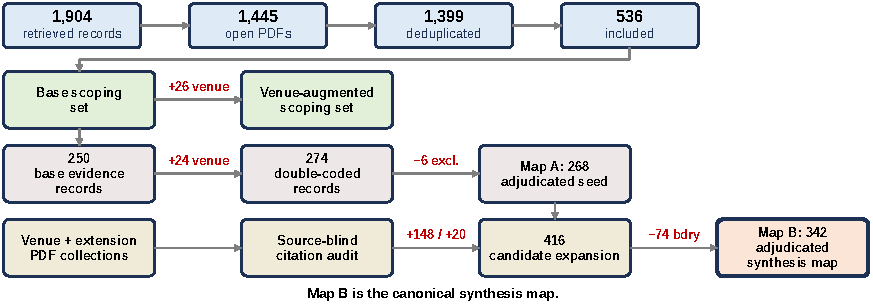
\includegraphics[width=\textwidth]{figures/generated/fig_corpus_lineage.pdf}%
\caption{Corpus lineage. Red deltas on the connectors are, in order, $+26$ and
$+24$ venue-linked additions, $-6$ exclusions, $+148$ new and $+20$ enriched
rows from the citation audit, and $-74$ boundary rows removed at adjudication.
The 416-row venue-expanded candidate map is second-coded and adjudicated into
Map~B (342 rows), the canonical synthesis evidence map. Map~A (268 rows) is the
double-coded adjudicated seed used for IAA and adjudication audit; the base and
venue-augmented scoping sets are used only for boundary checks, while a separate
300-paper source-blind citation audit over the venue and extension PDF
collections decides which papers enter the main text, case studies, or
appendix.}
\label{fig:corpus-flow}
\end{figure*}

\begin{table*}[t]
\centering
\small
\begin{tabularx}{\linewidth}{p{0.18\linewidth}p{0.16\linewidth}X}
\toprule
\textbf{Stage} & \textbf{Count} & \textbf{Rule} \\
\midrule
Initial retrieval & 1,904 records & Keyword search over arXiv, ACL Anthology, OpenReview, USENIX, AAAI/ACM landing pages where open versions were available, plus curated robust/trustworthy RAG paper lists; search cutoff 2026-06-03. \\
Open full-text corpus & 1,445 PDFs & Downloaded only open PDFs; removed failed downloads, inaccessible files, and non-PDF artifacts. \\
Deduplicated candidates & 1,399 papers & Deduplicated by normalised title and arXiv/proceedings identifiers; retained the most complete metadata record when preprint and proceedings versions overlapped. \\
Relevance screening & 536 included papers & Included papers that study RAG robustness, reliability, uncertainty, calibration, faithfulness, attack/defense, or evaluation under unreliable evidence; excluded application-only RAG papers. \\
Core pool & 112 papers & Papers directly shaping the taxonomy, threat/failure model, intervention mechanisms, or evaluation framework. \\
Core reading set & 100 papers & Core papers used as main narrative anchors; the remaining 12 core-pool papers stay in the broader scoping set. \\
Base scoping set & 300 papers & Core papers plus representative supporting work across all taxonomy branches before venue follow-up triage. \\
Venue-augmented scoping set & 326 papers & Base scoping set plus 26 venue-linked additions after follow-up triage. \\
Candidate evidence records & 274 papers & Base evidence map of 250 papers plus 24 venue-linked additions, double-coded and adjudicated. \\
Map A adjudicated seed & 268 papers & Candidate evidence records retained after final adjudication; used for IAA/adjudication provenance. \\
Map-B candidate expansion & 416 papers & Map A plus 148 source-blind human-citation-audit additions and 20 enriched original rows; used for second-coding review. \\
Map B adjudicated synthesis map & 342 papers & Map A plus 74 retained additions after second coding and final adjudication; frozen for current descriptive statistics. Post-freeze discoveries enter a recall log until a new version is coded. \\
\bottomrule
\end{tabularx}
\caption{Screening-flow summary. Search ends on 2026-06-03; coding and adjudication artifacts freeze on 2026-06-15. The supplement provides query strings, source counts, rules, exclusions, hashes, and a post-freeze recall log.}
\label{tab:review-protocol}
\end{table*}

\begin{table*}[t]
\centering
\scriptsize
\renewcommand{\arraystretch}{0.9}
\begin{tabularx}{\linewidth}{>{\raggedright\arraybackslash}p{0.22\linewidth}>{\raggedright\arraybackslash}p{0.16\linewidth}>{\raggedright\arraybackslash}p{0.25\linewidth}X}
\toprule
\textbf{Map-B field group} & \textbf{Coverage} & \textbf{Coding / audit source} & \textbf{Use and caveat} \\
\midrule
Canonical identifiers and source flags & 342/342 title, year, URL, source stratum, Map-A membership, Map-B version, core-reading flag & Deterministic merge from Map A, the venue/extension pools manifests, source-blind citation-audit decisions, and second-coding adjudication. & Defines the canonical adjudicated row set and source strata. \\
Core taxonomy fields & 342/342 failure type, taxonomy categories, method family, intervention point, contribution note, limitation note & Map-A adjudicated labels for original rows; second coding adjudicated labels for retained additions. & Used for Map-B synthesis and sensitivity counts. \\
Task / metric metadata & High coverage after adjudication & Map-A labels plus human-audit rationales and manifest metadata for retained additions. & Missing rows are not imputed for metric-level claims. \\
Author / venue metadata & Source/venue strata complete; author metadata incomplete for some additions & Proceedings metadata and paper manifests. & Venue/source strata are complete; author normalization remains an artifact-release cleanup item. \\
Human-audited rows retained in Map B & 94 retained rows with human citation-audit metadata & 74 retained additions plus 20 enriched Map-A rows. & Citation-audit metadata supports source-stratified synthesis; 74 excluded candidate additions remain in the release as boundary rows. \\
Second-coding/adjudication boundary & Map A: 274 candidates $\rightarrow$ 268 adjudicated rows; Map-B additions: 148 candidates $\rightarrow$ 74 retained additions & Map A has two-source independent coding and final adjudication; Map-B additions have independent second coding and final adjudication. & Second-coding agreement is strong, and adjudication is now applied to the canonical 342-row Map B. \\
\bottomrule
\end{tabularx}
\caption{Coding protocol and field coverage for the 342-row adjudicated Map B. The table separates Map-A adjudicated IAA, source-blind citation-audit metadata, and the second-coding/adjudication pass over the 148 candidate additions.}
\label{tab:map-b-coding-coverage}
\end{table*}

\begin{table*}[t]
\centering
\scriptsize
\renewcommand{\arraystretch}{0.92}
\begin{tabularx}{\linewidth}{>{\raggedright\arraybackslash}p{0.20\linewidth}>{\raggedright\arraybackslash}p{0.15\linewidth}>{\raggedright\arraybackslash}p{0.30\linewidth}X}
\toprule
\textbf{Artifact / set} & \textbf{Count} & \textbf{Count definition} & \textbf{Use in this paper} \\
\midrule
Map-A double-coded candidates & 274 & Candidate records coded by two human sources before final inclusion adjudication. & Used for human-human agreement and adjudication; six records were excluded from Map A. \\
Map A adjudicated seed & 268 & Included records after adjudication: 42 venue/proceedings-linked, 222 arXiv-only or emerging preprints, 2 preprints with year tags, 1 review-platform record, and 1 other/uncategorized record. & Used as the IAA/adjudication provenance snapshot, not the current synthesis denominator. \\
Venue-augmented scoping set & 326 & Original base scoping set plus 26 triaged venue-linked additions. & Used for broader scoping and boundary checks; not all rows are evidence-map records. \\
Source-blind citation audit & 300 & Human citation decisions over venue PDFs and extension PDFs. & Determines which audited papers enter the main text, case studies, appendix, background, or exclusion set; distinct from the base scoping set. \\
Map-B candidate expansion & 416 & Map A plus 148 candidate additions supported by the source-blind citation audit; 20 original rows enriched with citation-audit metadata. & Pre-adjudication expansion candidate map used for second-coding review. \\
Map B adjudicated synthesis map & 342 & Map A plus 74 retained additions after second coding and final adjudication. & Current evidence map for source-stratified synthesis and Map-B cross-tabs. \\
\bottomrule
\end{tabularx}
\caption{Reconciliation of reported corpus counts. The 342-row adjudicated Map B is the canonical synthesis map; Map A and the 274-candidate set are retained to report double-coding and adjudication provenance.}
\label{tab:source-strata-reconciliation}
\end{table*}


\FloatBarrier
\end{document}
